\documentclass[11pt,a4paper]{article}
\usepackage[french]{babel}
\usepackage[utf8]{inputenc}
\usepackage{mathtools,amssymb,amsthm}
\usepackage{mathrsfs,stmaryrd}
\usepackage{fancybox,mdframed,multicol,comment,enumitem}
\usepackage{microtype}

\usepackage{hyperref}
\hypersetup{
    colorlinks=true,       % false: boxed links; true: colored links
    linkcolor=blue,          % color of internal links
    citecolor=blue,        % color of links to bibliography
    filecolor=blue,      % color of file links
    urlcolor=black           % color of external links
}

%\usepackage[dvipsnames]{xcolor}

\usepackage[normalem]{ulem} % pour souligner avec changements de ligne
\usepackage{pgf,pgfmath,tikz}
\usetikzlibrary{arrows}
\usetikzlibrary[patterns]
\tikzset{every picture/.style={execute at begin picture={
   \shorthandoff{:;!?};}
}}

\newcommand*\circled[1]{\tikz[baseline=(char.base)]{
            \node[shape=circle,draw,inner sep=2pt] (char) {#1};}}


\def\point{node {$\bullet$}}

\usepackage{tkz-euclide}



\theoremstyle{definition}
\newtheorem{theoreme}{Théorème}[section]
\newtheorem{definition}[theoreme]{Définition}
\newtheorem{definitions}[theoreme]{Définitions}
\newtheorem{lemme}[theoreme]{Lemme}
\newtheorem{proposition}[theoreme]{Proposition}
\newtheorem{corollaire}[theoreme]{Corollaire}
\newtheorem{remarque}[theoreme]{Remarque}
\newtheorem{ex}{Problème}

\newcommand{\N}{\mathbb N}
\newcommand{\Z}{\mathbb Z}
\newcommand{\Q}{\mathbb Q}
\newcommand{\R}{\mathbb R}
\newcommand{\C}{\mathbb C}
\newcommand{\U}{\mathbb U}
\newcommand{\F}{\mathbb F}
\newcommand{\G}{\mathbb G}

\newcommand*{\etoile}
{
\begin{center}
$\star$\par
$\star$\hspace*{3ex}$\star$
\end{center}
}

\newcommand{\ensemble}[2]{\left \{ #1  
    \ifx&#2&%
       %
    \else%
       \, \middle | \, #2%
    \fi%
\right \}}

\newcommand{\modulo}[1]{\:\left(\operatorname{mod}\:#1\right)}

% délimiteurs

\DeclarePairedDelimiter{\abs}{\lvert}{\rvert}
\DeclarePairedDelimiter{\ceil}{\lceil}{\rceil}
\DeclarePairedDelimiter{\floor}{\lfloor}{\rfloor}


%%%%%%%%%%%%%%%%%%%%%%%%%%%%%%%%%
%%%%%% MISE EN FORME CLUB %%%%%%%
%%%%%%%%%%%%%%%%%%%%%%%%%%%%%%%%%

\pagestyle{empty}

\usepackage[margin=2.5cm]{geometry}
\everymath{\displaystyle}
\usepackage{fourier}
%\usepackage{fourier,eulervm}% Adobe Utopia et Euler
% En-tête des feuilles :

\newcommand{\enTete}[1]{
\noindent \textbf{\textsf{\href{http://depmath-nancy.univ-lorraine.fr/club/}{Club Mathématique de Nancy} \hfill Institut Élie Cartan}}
\hrule
\begin{center}
{\Huge \textbf{#1}}
\end{center}
\hrule
\vspace{1em}
}

\newcommand{\avertissement}{\begin{mdframed}[linewidth=1pt]\textbf{AVERTISSEMENT ! Ce document est un brouillon qui sert de catalogue pour les feuilles d'exos du club mathématique de Nancy \url{https://dmegy.perso.math.cnrs.fr/club/}. Ne pas diffuser tel quel aux élèves ni de façon large sur le net, il reste des coquilles et énoncés parfois peu précis. Ce document a vocation a rester inachevé. Il peut néanmoins être utile aux enseignants. Enfin, ce document change en permanence, la version à jour est récupérable sur \url{https://github.com/dmegy/clubmath-exos}.}\end{mdframed}}




% - - - - - - - - - - - - - -
% PARAMETRAGE DU PACKAGE ANSWERS 
% POUR LES INDICATIONS ET CORRECTIONS
% - - - - - - - - - - - - - - 

\usepackage{answers}

\Newassociation{sol}{Soln}{solutions}
% ira dans le fichier d'identifiant 'solutions'
% et écrira les solutions dans un environnement 'Soln'
\Newassociation{hint}{Hint}{indications}

\newenvironment{exo}{\begin{ex} \label{enonce.\theex} }{\end{ex} }

\renewenvironment{Soln}[1]{\noindent{\bf Correction de l'exercice \ref{enonce.#1}.} \\ }

\renewenvironment{Hint}[1]{ \noindent{\bf Exercice  \ref{enonce.#1}.} \label{hint.#1}}


% - - - - - - - - - - - - - - 
% FIN PARAMETRAGE ANSWERS
% - - - - - - - - - - - - - - 

%-----------------------------
% MACROS POUR LES FEUILLES DE TD


\newenvironment{feuilleTD}{


\Opensolutionfile{indications}[\jobname_hints]
\Opensolutionfile{solutions}[\jobname_sol]
}{
\Closesolutionfile{indications}
\Closesolutionfile{solutions}
}

\newcommand{\indications}{
\newpage
\noindent {\Large \bf Indications} \hrulefill

\vspace{1em}
\Readsolutionfile{indications}
}

\newcommand{\correction}{
\newpage
\hrule
\begin{center}
{\Large \bf Correction}
\end{center}
\hrule
\vspace{1em}
\Readsolutionfile{solutions}
}




\begin{document}
\Opensolutionfile{indications}[_\jobname_hints]
\Opensolutionfile{solutions}[_\jobname_sol]


\title{Autour du théorème de Pythagore}
\author{Damien Mégy}
\maketitle

\avertissement 

(Les exercices sont faisables sans connaître le concept de cosinus ni de sinus, uniquement avec Pythagore, à part les exceptions mentionnées à la fin.)

\tableofcontents



%Rajouter \url{https://twitter.com/maliuhudmuaz/status/1315383186852118530} utilse les demi-cercles.

\section{Échauffement, calculs concrets}

\begin{exo}
Soit $ABCD$ un trapèze rectangle comme sur la figure.
Calculer la longueur $AD$.
\begin{center}
\begin{tikzpicture}[scale=2,rotate=90,scale=.6]
\tkzDefPoint(2,3){A} \tkzDefPoint(2,0){B}  \tkzDefPoint(0,0){C}   \tkzDefPoint(0,1){D}  
\tkzDrawPolygon[very thick](A,B,C,D)
\tkzMarkRightAngles[size=.2](A,B,C B,C,D)
\tkzLabelSegment(A,B){$3$}
\tkzLabelSegment(B,C){$2$}
\tkzLabelSegment(C,D){$1$}
\end{tikzpicture}
\end{center}
\end{exo}

\begin{exo}
On considère une ligne brisée $ABCDE$ avec des angles droits et des distances comme sur la figure.
Calculer la distance $AE$.
\begin{center}
\begin{tikzpicture}[rotate=-50]
\tkzDefPoint(0,0){A}
\tkzDefPoint(1,0){B}
\tkzDefPoint(1,2){C}
\tkzDefPoint(4,2){D}
\tkzDefPoint(4,6){E}
\tkzMarkRightAngles[size=.2](A,B,C B,C,D C,D,E)
\tkzDrawSegments[very thick](A,B B,C C,D D,E)
\tkzLabelSegment[below left](A,B){$1$}
\tkzLabelSegment(B,C){$2$}
\tkzLabelSegment(C,D){$3$}
\tkzLabelSegment(D,E){$4$}
\tkzDrawPoints(A,B,C,D,E)
\tkzLabelPoints[left](A)\tkzLabelPoints[below](B)\tkzLabelPoints[above](C)\tkzLabelPoints[below](D)\tkzLabelPoints[right](E)

\end{tikzpicture}
\end{center}
\begin{hint}
Trouver un rectangle dont $[AE]$ est une diagonale et appliquer Pythagore.
\end{hint}
\begin{sol}
Considérons un point $P$ tel que $BCDP$ est un rectangle. Alors $APE$ est rectangle en $P$.
On a alors $AE^2 = (1+3)^2+(2+4)^2=4^2+6^2=52$, d'où $AE=2\sqrt{13}$.
\end{sol}
\end{exo}

%TODO : Double Pythagore : \url{https://www.youtube.com/watch?v=izbTPRWuO50} (facile)
% ou mettre la spirale directement...



\begin{exo}
Dans un demi-cercle de rayon $1$cm, on inscrit un autre demi-cercle plus petit, comme sur la figure.
Quel est le rayon du petit demi-cercle ?
\begin{center}
\begin{tikzpicture}[scale=2]
\tkzDefPoint(0,0){O} \tkzDefPoint(1,0){A}  \tkzDefPoint(-1,0){B}  
\tkzDefPoint(0,1/sqrt{2}){O'} \tkzDefPoint(1/sqrt{2},1/sqrt{2}){C}\tkzDefPoint(-1/sqrt{2},1/sqrt{2}){D}
\tkzDrawSemiCircle[black](O',D)
\tkzDrawSemiCircle[black,very thick](O,A)
\tkzDrawSegment[very thick](A,B)
\tkzDrawSegment(C,D)
\end{tikzpicture}
\end{center}
\end{exo}



\begin{exo}
Deux carrés identiques de $1\mathrm{cm}^2$ sont juxtaposés et inscrits dans un cercle, comme sur la figure.
Quel est le rayon du cercle ?
\begin{center}
\begin{tikzpicture}
\draw (2,1) -- (-2,1) -- (-2,-1) -- (2,-1) -- cycle;
\draw (0,1) -- (0,-1);
\draw[very thick] (0,0) circle (2.2360679775); % racine de 5...
\end{tikzpicture}
\end{center}
\begin{hint}

\end{hint}
\begin{sol}

\end{sol}
\end{exo}





\begin{exo}[Le triangle $30^\circ-60^\circ-90^\circ$]
Le triangle $ABC$ a des angles qui mesurent $30^\circ$, $60^\circ$ et $90^\circ$.
Son hypoténuse $AB$ mesure $1$ cm.
Quelle est la longueur des deux autres côtés ?
\begin{center}
\begin{tikzpicture}[scale=2.5]
\tkzDefPoint(0,1){B} \tkzDefPoint(sqrt{3},0){A} \tkzDefPoint(0,0){C}
\tkzDefBarycentricPoint(A=1,B=1,C=1)\tkzGetPoint{G}
\tkzDrawPolygon[very thick](A,B,C)
\tkzMarkRightAngle(A,C,B)
\tkzLabelSegment[above right](A,B){$1$}
\tkzLabelSegment[below](C,A){?} \tkzLabelSegment[left](B,C){?}
\tkzLabelAngle[pos=.3](C,B,A){$60^\circ$}
\end{tikzpicture}
\end{center}
\begin{hint}
Considérer la symétrie axiale d'axe $(AC)$.
\end{hint}
\begin{sol}
On obtient un triangle équilatéral quand on dédouble le triangle suivant l'axe proposé. On en déduit qu'un côté mesure $1/2$, et ensuite Pythagore donne $\sqrt{1-\frac14} = \frac{\sqrt 3}{2}$ pour le troisième côté.
\end{sol}
\end{exo}





\begin{exo}[Trois carrés dans un triangle équilatéral]
Trois carrés identiques de $1\mathrm{cm}^2$ sont placés dans un triangle équilatéral comme sur la figure.
Combien mesure le triangle équilatéral ?
\begin{center}
\begin{tikzpicture}
\tkzDefPoint(0,0){A}\tkzDefPoint(1,0){B}
\tkzDefSquare(A,B)\tkzGetPoints{C}{D}
\tkzDrawPolygon(A,B,C,D)

\tkzDefPoint(3/2,0){E}\tkzDefPoint(3/2+sqrt{3}/2,1/2){F}
\tkzDefSquare(E,F)\tkzGetPoints{G}{H}
\tkzDrawPolygon(E,F,G,H)

\tkzDefPoint(3/4,1+3*sqrt{3}/4){I} \tkzDefPoint(1/4,1+sqrt{3}/4){J}
\tkzDefSquare(I,J)\tkzGetPoints{K}{L}
\tkzDrawPolygon(I,J,K,L)

\tkzDefPoint(-1/sqrt{3},0){X}\tkzDefPoint(3/2+2/sqrt{3},0){Y}
\tkzDefTriangle[equilateral](X,Y) \tkzGetPoint{Z}
\tkzDrawPolygon[very thick](X,Y,Z)

\end{tikzpicture}
\end{center}
\begin{hint}
Le triangles qui apparaissent sont tous des triangles rectangles ayant des angles de $30^\circ$ et $60^\circ$, dont on sait calculer les côtés.
\end{hint}
\begin{sol}
On trouve $\frac{1}{\sqrt 3}+1+\frac12+\frac{2}{\sqrt 3} = \frac32+\sqrt 3$.
\end{sol}
\end{exo}


\begin{exo}
Soit $ABCD$ un quadrilatère. Montrer que les deux propositions suivantes sont équivalentes:
\begin{enumerate}
\item $ABCD$ est un rectangle.
\item Pour tout point $X$ du plan, on a $AX^2+CX^2 = BX^2+DX^2$.
\end{enumerate}
\begin{hint}
Pour $2\implies 1$, on peut prendre des points $P$ particuliers.
\end{hint}
\end{exo}



\begin{exo}[Périmètre et diagonale]
% note : on a pris le triangle $3-4-5$ et on a doublé les dimensions pour que ça crève moins les yeux.
Un rectangle a un diagonale de $10$ mètres et un périmètre de $28$ mètres. Calculer sa largeur et sa longueur.
\begin{center}
\begin{tikzpicture}[scale=.5]
\draw[very thick] (0,0) rectangle (8,6) ;
\draw (0,0) -- (8,6) node[midway,fill=white] {$10$};
\end{tikzpicture}
\end{center}
\begin{hint}
La largeur et la longueur sont des nombres entiers.
\end{hint}
\begin{sol}
On a d'après Pythagore $\ell^2+L^2=10^2=100$ et $28=p=2\ell+2L$ donc $\ell+L=14$.

On en déduit $(\ell+L)^2=14^2=196$ et donc en soustrayant, $L\times \ell = 48$.

D'après l'indication, la largeur et la longueur sont des nombres entiers.
En procédant par tâtons, on trouve $l=6$ et $L=8$.
Sans utiliser l'indication, on peut remplacer $L$ par $14-\ell$, remplacer dans la seconde équation et résoudre le trinôme.
\end{sol}
\end{exo}




Dans toute la suite, un triangle \og $3-4-5$\fg{} est un triangle dont les côtés mesurent $3$cm, $4$cm et $5$cm. C'est un triangle rectangle, comme on peut le vérifier à l'aide du théorème de Pythagore.


% - - - - -


\begin{exo}
On inscrit cinq cercles identiques dans un carré, comme sur la figure.
Sachant que le rayon des cercles est égal à $1cm$, quelles sont les dimensions du carré ?
\begin{center}
\begin{tikzpicture}
\def\sqrtt{1.4142135624}
\draw[very thick] (-\sqrtt-1,-\sqrtt-1) rectangle (1+\sqrtt,1+\sqrtt) ;
\draw (0,0) circle( 1);
\draw (\sqrtt,\sqrtt) circle( 1);
\draw (\sqrtt,-\sqrtt) circle( 1);
\draw (-\sqrtt,\sqrtt) circle( 1);
\draw (-\sqrtt,-\sqrtt) circle( 1);
\end{tikzpicture}
\end{center}
\begin{hint}
Tracer une diagonale du carré : combien mesure-t-elle ?
\end{hint}
\begin{sol}
La diagonale mesure $d=4+2\sqrt 2$.
On en déduit que le côté du carré est égal à  :
\[ c = \frac{d}{\sqrt 2} = 2\sqrt 2+2.\]
\end{sol}
\end{exo}






\begin{exo}
Soit $ABC$ un triangle rectangle en $A$ dont l'hypoténuse mesure $4$cm.
On la partage en quatre segments égaux $[BP]$, $[PQ]$, $[QR]$ et $[RC]$.
Calculer $AP^2+AQ^2+AR^2$.
Dans le cas général où l'hypoténuse est de longueur $\ell$, calculer $AP^2+AQ^2+AR^2$ en fonction de $\ell$.
\begin{center}
\begin{tikzpicture}[scale=.7]
\tkzDefPoint(0,0){A}\tkzDefPoint(0,4){B}\tkzDefPoint(8,0){C}
\tkzDrawPolygon[very thick](A,B,C)
\tkzDefPoint(2,3){P}\tkzDefPoint(4,2){Q}\tkzDefPoint(6,1){R}
\tkzDrawPoints(P,Q,R)
\tkzLabelPoint[above right](P){$P$}\tkzLabelPoint[above right](Q){$Q$}\tkzLabelPoint[above right](R){$R$}
\tkzLabelPoint[above](B){$B$}\tkzLabelPoint[right](C){$C$}\tkzLabelPoint[below left](A){$A$}
\tkzDrawSegments(A,P A,Q A,R)
\tkzMarkSegments[mark=||](B,P P,Q Q,R R,C)
\tkzMarkRightAngle(C,A,B)
\end{tikzpicture}
\end{center}
\begin{hint}
Pour le cas particulier on trouve $14$.
\end{hint}
\begin{sol}
On \og quadrille \fg{}, c'est-à-dire qu'on projette les points $P$, $Q$ et $R$ sur $(AB)$ et $(AC)$. Ensuite on applique plusieurs fois Pythagore.
Cas général : $\frac{7}{8}BC^2$.
\end{sol}
\end{exo}





\begin{exo}
% source : chaîne PreMath : https://www.youtube.com/watch?v=_WhmxcPQX4U 
Dans deux demi-cercles identiques, on inscrit d'une part un rectangle $ABCD$ formé de quatre petits carrés juxtaposés, et d'autre part un carré $EFGH$.
Lequel de $ABCD$ et $EFGH$ a la plus grande aire ?

\begin{center}
\begin{tikzpicture}
\tkzDefPoint(-2,1){A} \tkzDefPoint(-2,0){B}
\tkzDefPoint(2,0){C} \tkzDefPoint(2,1){D}
\tkzDrawPolygon(A,B,C,D)
\draw  (-1,0) -- (-1,1);
\draw  (0,0) -- (0,1);
\draw  (1,0) -- (1,1);
\tkzDefPoint(0,0){O}
\tkzDefPoint(-sqrt{5},0){P}
\tkzDefPoint(sqrt{5},0){Q}
\tkzDrawSemiCircle[black, very thick](O,Q)
\tkzDrawSegment(P,Q)
\tkzDrawPoints(A,B,C,D)
\tkzLabelPoints[above left](A) \tkzLabelPoints[below](B) \tkzLabelPoints[below](C) \tkzLabelPoints[above right](D)
\end{tikzpicture}
\hspace{1cm}
\begin{tikzpicture}
\tkzDefPoint(-1,2){E} \tkzDefPoint(-1,0){F}
\tkzDefPoint(1,0){G} \tkzDefPoint(1,2){H}
\tkzDrawPolygon(E,F,G,H)
\tkzDefPoint(0,0){O}
\tkzDefPoint(-sqrt{5},0){P}
\tkzDefPoint(sqrt{5},0){Q}
\tkzDrawSemiCircle[black, very thick](O,Q)
\tkzDrawSegment(P,Q)
\tkzDrawPoints(E,F,G,H)
\tkzLabelPoints[above left](E) \tkzLabelPoints[below](F) \tkzLabelPoints[below](G) \tkzLabelPoints[above right](H)
\end{tikzpicture}
\end{center}
\begin{sol}
En appliquant le théorème de Pythagore, on voit que les deux aires sont égales  à $\dfrac 45 R^2$ !
\end{sol}

\end{exo}






\begin{exo}
On considère deux cercles de rayon $2$cm et $3$cm qui ont un unique point de contact entre eux.
Ils sont tous deux tangents en $P$ et $Q$ à une certaine droite.
Quelle est la distance $PQ$ ?
\begin{center}
\begin{tikzpicture}[scale=.7]
\tkzDefPoint(0,2){O}\tkzDefPoint(sqrt{24},3){O'}
\tkzDefPoint(0,0){P}\tkzDefPoint(sqrt{24},0){Q}
\tkzDrawCircle[black,thick](O,P)
\tkzDrawCircle[black,thick](O',Q)
\tkzDrawLine(P,Q)
\tkzDrawPoints(P,Q)
\tkzLabelPoints(P,Q)
\end{tikzpicture}
\end{center}
\begin{hint}
\end{hint}
\begin{sol}
\end{sol}
\end{exo}



\begin{exo}
% pythagore 2 fois, simples
Dans la figure ci-dessous, le segment $[PR]$ est un diamètre du cercle.
Si $PQ=7$, $QR=6$ et $RS=2$, que vaut le périmètre du quadrilatère $PQRS$ ?
\begin{center}

\begin{tikzpicture}[line cap=round,line join=round,>=triangle 45,scale=.8]
\clip(-3.5797558586948437,-3.881851674112303) rectangle (4.125414120251267,3.396782109570719);
\draw [very thick] (0.,0.) circle (3.cm);
\draw [very thick] (-3.,0.)-- (3.,0.);
\draw [very thick] (3.,0.)-- (0.5768677789417458,2.9440148718406327);
\draw [very thick] (0.5768677789417458,2.9440148718406327)-- (-3.,0.);
\draw [very thick] (3.,0.)-- (2.6083696721783043,-1.482028222828582);
\draw [very thick] (2.6083696721783043,-1.482028222828582)-- (-3.,0.);

\draw [fill=black] (0.,0.) circle (2.0pt);
\draw[color=black] (0.025162952883515128,0.3353529661501663) node {$O$};
\draw [fill=black] (3.,0.) circle (2.5pt);
\draw[color=black] (3.2585824976198294,0.06016832404494808) node {$R$};
\draw [fill=black] (-3.,0.) circle (2.0pt);
\draw[color=black] (-3.3320896808001472,0.10144602036073082) node {$P$};
\draw [fill=black] (0.5768677789417458,2.9440148718406327) circle (2.5pt);
\draw (0.6718468618307779,3.197273244044436) node {$Q$};
\draw (1.896418519198999,1.7) node {6};
\draw (-1.4057971860636196,1.614961551939431) node {7};
\draw [fill=black] (2.6083696721783043,-1.482028222828582) circle (2.5pt);
\draw (2.8595647665672628,-1.5496618322705786) node {$S$};
\draw (2.6256578207778274,-0.6965894417444021) node {2};
\draw (-0.27754015343222493,-0.94) node {?};
\end{tikzpicture}
\end{center}
\end{exo}



\begin{exo}
Les diagonales du losange ci-dessous mesurent $6\,$cm et $8\,$cm. 
Combien mesure la hauteur marquée sur la figure ?
\begin{center}
\begin{tikzpicture}[scale=.7,rotate=atan(3/4)]
\tkzDefPoint(0,0){O}
\tkzDefPoint(-4,0){A}
\tkzDefPoint(0,3){B}
\tkzDefPoint(4,0){C}
\tkzDefPoint(0,-3){D}
\tkzDrawSegments[very thick](A,B B,C C,D D,A)
\tkzDefPointBy[projection=onto A--D](B)
 \tkzGetPoint{H}
\tkzDrawSegment(B,H)
\tkzAutoLabelPoints[center = O,dist= .1](A,B,C,D,H)
\tkzMarkRightAngles(D,H,B)
\end{tikzpicture}

\end{center}

\end{exo}


\begin{exo}
Combien mesure le segment $[DF]$ ?
\begin{center}
\begin{tikzpicture}[line cap=round,line join=round,>=triangle 45,scale=.6,rotate=40]

\draw[very thick] (-0.4242640687119284,4.) -- (-0.4242640687119285,3.5757359312880714) -- (0.,3.5757359312880714) -- (0.,4.) -- cycle; 
\draw[very thick] (0.4242640687119284,0.) -- (0.42426406871192845,0.4242640687119284) -- (0.,0.4242640687119284) -- (0.,0.) -- cycle; 
\draw[very thick] (-1.1421023839543198,5.783993283625307) -- (-0.8482507356267196,5.477968433694534) -- (-0.5422258856959464,5.771820082022135) -- (-0.8360775340235467,6.0778449319529075) -- cycle; 
\draw[very thick] (-3.,4.)-- (0.,4.);
\draw[very thick] (0.,4.)-- (0.,0.);
\draw[very thick] (0.,0.)-- (5.,0.);
\draw[very thick](-3.,4.)-- (-0.8360775340235467,6.0778449319529075);
\draw[very thick] (-0.8360775340235467,6.0778449319529075)-- (5.,0.);

\draw [fill=black] (-3.,4.) circle (2.5pt);
\draw(-3.58,4.31) node {$A$};
\draw [fill=black] (0.,4.) circle (2.5pt);
\draw (0.36,3.73) node {$B$};
\draw [fill=black] (0.,0.) circle (2.0pt);
\draw  (-0.34,-0.21) node {$C$};
\draw [fill=black] (5.,0.) circle (2.5pt);
\draw (5.3,-0.31) node {$D$};
\draw(-1.52,3.77) node {3};
\draw (-0.26,2.03) node {4};
\draw (2.66,-0.29) node {5};
\draw [fill=black] (-0.8360775340235467,6.0778449319529075) circle (2.0pt);
\draw (-0.88,6.65) node {$F$};
\draw (-2.02,5.45) node {3};
\end{tikzpicture}
%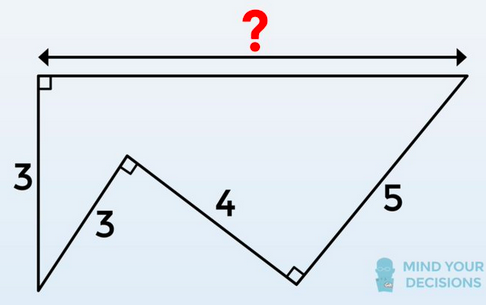
\includegraphics[scale=.4]{pythagore4.png}
\end{center}
\end{exo}



\begin{exo}
Le quadrilatère suivant est un trapèze. 
Les longueurs de ses côtés sont données sur la figure.
Quelle est son aire ?
\begin{center}
\begin{tikzpicture}[scale=.2]
\tkzDefPoint(0,0){A}
\tkzDefPoint(5,12){B}
\tkzDefPoint(15,12){C}
\tkzDefPoint(24,0){D}
%\tkzDefPoint(14,0)
\tkzDrawPolygon[very thick](A,B,C,D)
%\tkzdrawSegment(B,E)
\tkzLabelSegment[above left](A,B){$13$}
\tkzLabelSegment[above](B,C){$10$}
\tkzLabelSegment[above right](C,D){$15$}
\tkzLabelSegment[below](D,A){$24$}
\end{tikzpicture}
%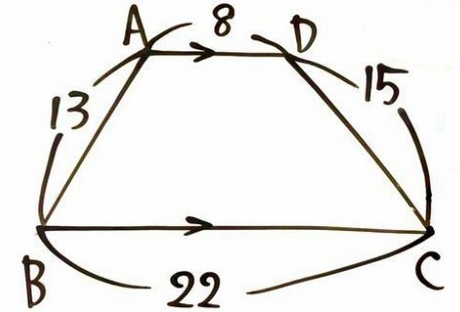
\includegraphics[scale=.4]{pythagore7.png}
\end{center}
\begin{sol}
\begin{center}
\begin{tikzpicture}[scale=.2]
\tkzDefPoint(0,0){A}
\tkzDefPoint(5,12){B}
\tkzDefPoint(15,12){C}
\tkzDefPoint(24,0){D}
\tkzDefPoint(14,0){E}
\tkzDefPoint(5,0){H}
\tkzDrawPolygon[very thick](A,B,C,D)
\tkzDrawSegment(B,E)
\tkzDrawSegment(B,H)
\tkzLabelSegment[above left](A,B){$13$}
\tkzLabelSegment[above](B,C){$10$}
\tkzLabelSegment[above right](C,D){$15$}
\tkzLabelSegment[below](D,A){$24$}
\end{tikzpicture}
%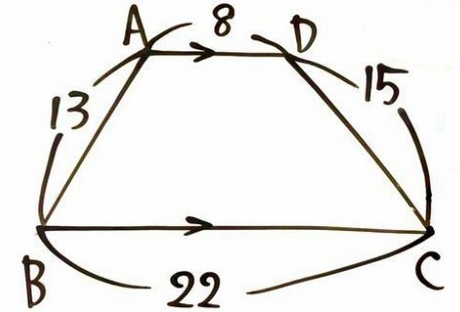
\includegraphics[scale=.4]{pythagore7.png}
\end{center}
\end{sol}
\end{exo}





\begin{exo}
Dans un triangle rectangle, le cercle inscrit touche l'hypoténuse en la divisant en deux segments de $3$ et $5$ cm.
Quelle est l'aire du triangle ?

\begin{center}
\begin{tikzpicture}

\end{tikzpicture}


\begin{tikzpicture}[line cap=round,line join=round,>=triangle 45,scale=.7]
\draw[very thick] (-0.5938096629462137,3.4597430801129723) -- (-0.30355274305918567,3.2578745078742624) -- (-0.10168417082047576,3.5481314277612905) -- (-0.3919410907075038,3.75) -- cycle; 
\draw [very thick] (0.,1.5677643628300215) circle (1.5677643628300215cm);
\draw [very thick] (-0.3919410907075038,3.75)-- (5.,0.);
\draw [very thick] (-3.,0.)-- (-0.3919410907075038,3.75);
\draw [very thick] (-3.,0.)-- (0.,0.);
\draw [very thick] (0.,0.)-- (5.,0.);
\draw [very thick,dash pattern=on 5pt off 5pt] (0.,1.5677643628300215)-- (0.,0.);


\draw [fill=black] (-3.,0.) circle (2.5pt);
\draw (-3.6,-0.01) node {$A$};
\draw [fill=black](0.,0.) circle (2.0pt);
\draw [fill=black](5.,0.) circle (2.5pt);
\draw (5.46,-0.17) node {$C$};
\draw[fill=black] (0.,1.5677643628300215) circle (2.5pt);
\draw (0.14,1.93) node {$O$};
\draw[fill=black] (-0.3919410907075038,3.75) circle (2.0pt);
\draw(-0.48,4.25) node {$D$};
\draw[color=black] (-1.44,-0.3) node {3};
\draw[color=black] (2.56,-0.3) node {5};
\draw[color=black] (-0.26,0.97) node {R};
\end{tikzpicture}
%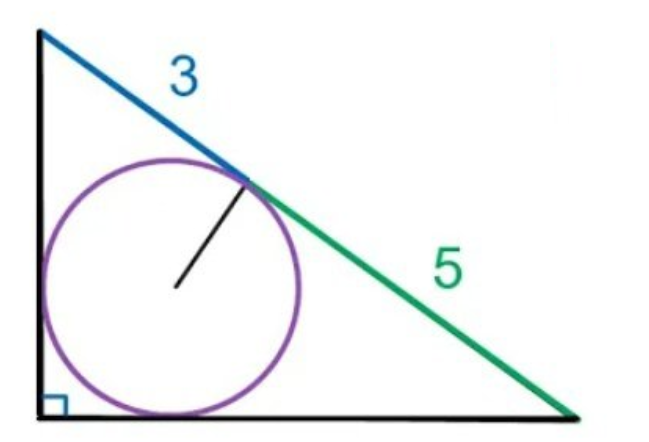
\includegraphics[scale=.4]{pythagore9.png}
\end{center}
%\emph{(Bonus : en déduire ensuite le rayon du cercle inscrit, puis les dimensions du triangle. Ceci n'est pas nécessaire pour trouver l'aire du triangle !)}
\begin{sol}
Pythagore donne $2r^2+16r=30$.

Or, en reliant $O$ aux sommets du triangle, on remarque que l'aire recherchée est $r^2+3r+5r=r^2+8r=15$.

En bonus, on peut trouver$R=-4+\sqrt{31}$ et calculer les dimensions du triangle, mais il n'y a pas besoin de ça pour trouver l'aire.
\end{sol}
\end{exo}




\begin{exo}[Spirale pythagoricienne]
Cette spirale est formée de triangles rectangles juxtaposés. On a 
$OA=AB=BC=CD= DE=EF=FG=GH=HI=1$.
Que vaut $OI$ ?
\begin{center}
%\definecolor{qqwuqq}{rgb}{0.,0.39215686274509803,0.}
\definecolor{qqwuqq}{rgb}{0,0,0}
\begin{tikzpicture}[line cap=round,line join=round,>=triangle 45,rotate=30,scale=1.2]
%\clip(-1.28,-3.08) rectangle (4.72,2.7);
%angles:
\draw[color=qqwuqq,fill=qqwuqq,fill opacity=0.10000000149011612] (0.28284271247461906,0.) -- (0.28284271247461906,0.28284271247461906) -- (0.,0.28284271247461906) -- (0.,0.) -- cycle; 
\draw[color=qqwuqq,fill=qqwuqq,fill opacity=0.10000000149011612] (0.2,0.8) -- (0.4,1.) -- (0.2,1.2) -- (0.,1.) -- cycle; 
\draw[color=qqwuqq,fill=qqwuqq,fill opacity=0.10000000149011612] (0.7549360435341675,1.428337411163077) -- (1.033705413557638,1.476166673510697) -- (0.9858761512100178,1.7549360435341674) -- (0.7071067811865475,1.7071067811865475) -- cycle; 
\draw[color=qqwuqq,fill=qqwuqq,fill opacity=0.10000000149011612] (1.5947420120656104,1.6108727725011909) -- (1.86007799947673,1.5129094437267652) -- (1.9580413282511557,1.7782454311378848) -- (1.692705340840036,1.8762087599123105) -- cycle; 
\draw[color=qqwuqq,fill=qqwuqq,fill opacity=0.10000000149011612] (2.4245267948738216,1.3363429000893319) -- (2.6180399842767828,1.1300599741669628) -- (2.824322910199152,1.3235731635699242) -- (2.6308097207961905,1.5298560894922932) -- cycle; 
\draw[color=qqwuqq,fill=qqwuqq,fill opacity=0.10000000149011612] (3.0476710481598275,0.7080978975204855) -- (3.1401089613180893,0.440786782504769) -- (3.407420076333806,0.5332246956630311) -- (3.314982163175544,0.8005358106787476) -- cycle; 
\draw[color=qqwuqq,fill=qqwuqq,fill opacity=0.10000000149011612] (3.359379289033147,-0.12909847315852738) -- (3.3439260622996714,-0.41151872346562524) -- (3.626346312606769,-0.4269719501991008) -- (3.6417995393402447,-0.1445516998920029) -- cycle; 
\draw[color=qqwuqq,fill=qqwuqq,fill opacity=0.10000000149011612] (3.328447719041178,-1.028752263517281) -- (3.214141911983702,-1.2874686767440788) -- (3.4728583252105,-1.4017744838015544) -- (3.5871641322679757,-1.1430580705747568) -- cycle; 



\draw[thick]  (1.,0.)-- (0.,0.);
\draw[thick]  (0.,1.)-- (1.,0.);
\draw[thick]  (0.,1.)-- (0.,0.);
\draw[thick] (1.,0.)-- (0.7071067811865475,1.7071067811865475);
\draw[thick]  (1.,0.)-- (1.692705340840036,1.8762087599123105);
\draw[thick]  (1.,0.)-- (2.6308097207961905,1.5298560894922932);
\draw[thick]  (1.,0.)-- (3.314982163175544,0.8005358106787476);
\draw[thick]  (1.,0.)-- (3.6417995393402447,-0.1445516998920029);
\draw[thick]  (1.,0.)-- (3.5871641322679757,-1.1430580705747568);
\draw[thick] (3.183032075771265,-2.057758721559405)-- (1.,0.);
\draw[thick]  (0.,1.)-- (0.7071067811865475,1.7071067811865475);
\draw[thick] (0.7071067811865475,1.7071067811865475)-- (1.692705340840036,1.8762087599123105);
\draw[thick]  (1.692705340840036,1.8762087599123105)-- (2.6308097207961905,1.5298560894922932);
\draw[thick] (2.6308097207961905,1.5298560894922932)-- (3.314982163175544,0.8005358106787476);
\draw[thick]  (3.314982163175544,0.8005358106787476)-- (3.6417995393402447,-0.1445516998920029);
\draw[thick] (3.6417995393402447,-0.1445516998920029)-- (3.5871641322679757,-1.1430580705747568);
\draw[thick]  (3.183032075771265,-2.057758721559405)-- (3.5871641322679757,-1.1430580705747568);


\draw[thick]  (0.,0.) node {$\bullet$};
\draw[thick]  (-0.36,0.09) node {$A$};
\draw[thick] (0.,1.) node {$\bullet$};
\draw[thick]  (-0.36,1.37) node {$B$};
\draw[thick] (1.,0.) node {$\bullet$};
\draw[thick]  (0.78,-0.35) node {$O$};
\draw[thick]  (0.7071067811865475,1.7071067811865475) node {$\bullet$};
\draw[thick]  (0.5,2.17) node {$C$};
\draw[thick]  (1.692705340840036,1.8762087599123105) node {$\bullet$};
\draw[thick]  (1.84,2.21) node {$D$};
\draw[thick]  (2.6308097207961905,1.5298560894922932) node {$\bullet$};
\draw[thick]  (2.78,1.85) node {$E$};
\draw[thick]  (3.314982163175544,0.8005358106787476) node {$\bullet$};
\draw[thick]  (3.46,1.13) node {$F$};
\draw[thick]  (3.6417995393402447,-0.1445516998920029) node {$\bullet$};
\draw[thick]  (3.78,0.19) node {$G$};
\draw[thick]  (3.5871641322679757,-1.1430580705747568) node {$\bullet$};
\draw[thick]  (3.88,-1.07) node {$H$};
\draw[thick]  (3.183032075771265,-2.057758721559405) node {$\bullet$};
\draw[thick] (3.54,-2.11) node {$I$};



\end{tikzpicture}
\end{center}
\begin{hint}
Appliquer Pythagore dans les triangles rectangles en partant du plus petit. Le résultat demandé est un nombre entier.
\end{hint}
\begin{sol}
\end{sol}
\end{exo}


\begin{exo}[Pythagore et triangles isocèles]
\url{https://www.youtube.com/watch?v=tbRtYT1bLNs}
Début avec Pythagore et triangles isocèles. Tronquer l'exo pour ne pas avoir besoin de trigo.
\end{exo}

% - - - - - - - - - - - - - - - - - - - - 

\begin{exo}% triangles égaux
Dans un carré $ABCD$, on trace un point $M$ sur le côté $[BC]$.
Les perpendiculaires à $(AM)$ passant par $D$ et $B$ coupent $(AM)$ en $P$ et $Q$.
Sachant que $DP=5$cm et $BQ=4$cm, déterminer l'aire du carré $ABCD$.%\\
%(Bonus : calculer ensuite la distance $AM$.)
% a besoin de triangles semblables ou de Thalès.
\begin{center}
\begin{tikzpicture}[rotate=atan(4/5), scale=.8]
\tkzDefPoint(0,0){A} \tkzDefPoint(5,-4){B} \tkzDefPoint(9,1){C} \tkzDefPoint(4,5){D}
\tkzDefBarycentricPoint(A=1,C=1)\tkzGetPoint{G}
\tkzDrawPolygon[very thick](A,B,C,D)
\tkzDefPoint(5+16/5,0){M} \tkzDefPoint(4,0){P}  \tkzDefPoint(5,0){Q}
\tkzDrawSegments(A,M D,P B,Q)
\tkzMarkRightAngle(D,P,A) \tkzMarkRightAngle(B,Q,M)
\tkzDrawPoints(P,Q,M)
\tkzLabelPoints[below left](A) \tkzLabelPoints[below right](B) \tkzLabelPoints[above right](C) \tkzLabelPoints[above left](D)
\tkzLabelPoints[right](M) \tkzLabelPoints[below](P)\tkzLabelPoints[above](Q)
\tkzLabelSegment[below left](D,P){$5$} \tkzLabelSegment[above right](B,Q){$4$} \tkzLabelSegment[left](A,D){?}
\end{tikzpicture}
\end{center}
\begin{hint}
Considérer les triangles $ADP$ et $AQB$
\end{hint}
\begin{sol}
Les triangles $ADP$ et $AQB$ sont égaux : ils ont les mêmes angles et la même hypoténuse.
On en déduit que $AP=4$ et $AQ=5$, et en appliquant le théorème de Pythagore, on trouve le côté du carré : $AB=\sqrt{41}$.
Le carré a donc une aire de $41\mathrm{cm}^2$.

Pour trouver la distance $AM$, il suffit de trouver $QM$. Le plus simple est d'utiliser des triangles semblables, ou Thalès, on trouve $QM=16/5$, donc $AM=5+16/5=41/5$.
\end{sol}
\end{exo}





% - - - - - - - -
\begin{exo}
On considère un triangle isocèle dont les côtés mesurent $13$cm, $13$cm et $10$cm.
Quel est le rayon de son cercle circonscrit ?
\begin{center}
\begin{tikzpicture}[scale=1/3]
\tkzDefPoint(0,0){H}\tkzDefPoint(-5,0){B}\tkzDefPoint(5,0){C}\tkzDefPoint(0,12){A}
\tkzDefCircle[circum](A,B,C) \tkzGetPoint{O} 
\tkzDrawCircle[very thick, black](O,A)
\tkzDrawPolygon(A,B,C)
\tkzLabelSegments[above left](A,B){$13$}\tkzLabelSegments(A,C){$13$}\tkzLabelSegments(B,C){$10$}
\end{tikzpicture}
\end{center}
\begin{hint}
Il y a une hauteur $h$ que l'on peut calculer à l'aide de Pythagore.
Ensuite, si l'on note $H$ le pied de cette hauteur et $O$ le centre du cercle circonscrit, on peut par exemple appliquer Pythagore dans le triangle rectangle $OHB$.
\end{hint}
\begin{sol}
On trouve une hauteur de $12$, et un rayon de $\frac{169}{24}$.
\end{sol}
\end{exo}




\begin{exo}[Zig-Zag dans un carré]
Que vaut  à chaque fois le côté du carré ?
\begin{center}
\begin{tikzpicture}[scale=1,rotate=30]
\draw[very thick] (0,0)  -- (1,0) node[midway, above] {$1$} 
-- (1,2) node[midway, right] {$2$}  
-- (4,2) node[midway, below] {$3$}  ;
\draw[very thick] (0,0) -- (1,3) -- (4,2) -- (3,-1) -- cycle;
\draw [black] (1,0) rectangle (.8,.2) ;
\draw [black] (1,2) rectangle (1.2,1.8) ;
\end{tikzpicture}
\hspace{1cm}
\begin{tikzpicture}[scale=.18,rotate=20]
\draw[very thick] (0,0)  -- (14,0) node[midway, above] {$14$} 
-- (14,7) node[midway, right] {$7$}  
-- (23,7) node[midway, below] {$9$}  ;
\draw[very thick] (0,0) -- (8,15) -- (23,7) -- (15,-8) -- cycle;
\draw [black] (13,0) rectangle (14,1) ;
\draw [black] (14,6) rectangle (15,7) ;
\end{tikzpicture}

\end{center}
\begin{hint}
\end{hint}
\begin{sol}
Le côté vaut $\sqrt{10}$.

Pour le second la source d'origine est : \url{https://twitter.com/0y6tr4/status/1522092641017602049}. Mais en fait le premier est mieux, plus simple
\end{sol}
\end{exo}



\begin{exo}
Une feuille de papier rectangulaire de dimensions $12\times 8$ est pliée de sorte que le coin de la feuille revienne exactement à la moitié du grand côté.
Quelle est la longueur du pli?
\begin{center}
\begin{tikzpicture}[line cap=round,line join=round,>=triangle 45,scale=.4]
\draw [very thick] (12.,8.)-- (12.,0.);
\draw [very thick] (0.,6.2741019624591665)-- (6.,8.);
\draw [very thick](8.301197383387779,0.)-- (0.,6.2741019624591665);
\draw [very thick] (6.,8.)-- (8.301197383387779,0.);
\draw [very thick] (0.,8.)-- (0.,6.2741019624591665);
\draw [very thick](8.301197383387779,0.)-- (12.,0.);
\draw [very thick,dash pattern=on 6pt off 6pt] (8.301197383387779,0.)-- (0.,0.);
\draw [very thick,dash pattern=on 6pt off 6pt] (0.,0.)-- (0.,6.2741019624591665);
\draw [very thick] (0.,8.)-- (6.,8.);
\draw [very thick] (2.935418600966369,8.154995357680713) -- (2.935418600966369,7.845004642319288);
\draw [very thick] (3.064581399033631,8.154995357680713) -- (3.064581399033631,7.845004642319288);
\draw [very thick] (6.,8.)-- (12.,8.);
\draw [very thick] (8.935418600966369,8.154995357680713) -- (8.935418600966369,7.845004642319288);
\draw [very thick] (9.064581399033631,8.154995357680713) -- (9.064581399033631,7.845004642319288);
\begin{scriptsize}
\draw [fill=black] (0.,0.) circle (2.0pt);
\draw (-0.5927513169194987,-0.0419588630298644) node {$C$};
\draw [fill=black] (12.,0.) circle (2.5pt);
\draw (12.168533132126012,0.4746923292391769) node {$D$};
\draw [fill=black] (12.,8.) circle (2.5pt);
\draw (12.168533132126012,8.482785809409318) node {$E$};
\draw [fill=black] (0.,8.) circle (2.5pt);
\draw (-0.3602582803984267,8.61194860747658) node {$F$};
\draw [fill=black] (0.,6.2741019624591665) circle (2.5pt);
\draw (-0.6185838765329512,6.2870182422658925) node {$G$};
\draw [fill=black] (6.,8.) circle (2.5pt);
\draw (6.175379301805044,8.482785809409318) node {$H$};
\draw [fill=black] (8.301197383387779,0.) circle (2.0pt);
\draw (8.293649190108145,-0.5327774956854536) node {$I$};
\end{scriptsize}
\end{tikzpicture}
\end{center}
\end{exo}




\begin{exo}
Dans la figure ci-dessous, une ligne brisée $ABCD$ dont les angles sont droits est inscrite dans un quart de cercle de centre $O$.
Si $AB=12$ et $BC=2$, que vaut le rayon du cercle ? % 10
\begin{center}
\definecolor{xdxdff}{rgb}{0.49019607843137253,0.49019607843137253,1.}
\definecolor{uuuuuu}{rgb}{0.26666666666666666,0.26666666666666666,0.26666666666666666}
\definecolor{ududff}{rgb}{0.30196078431372547,0.30196078431372547,1.}
\begin{tikzpicture}[line cap=round,line join=round,>=triangle 45,x=1.0cm,y=1.0cm]
\clip(-1.02,-1.08) rectangle (5.18,4.86);
\draw [very thick] (0.,4.)-- (3.8415567807131086,1.1146485995851507);
\draw [very thick](3.8415567807131086,1.1146485995851507)-- (3.363454090563979,0.47810269014912943);
\draw [very thick] (3.363454090563979,0.47810269014912943)-- (4.,0.);
\draw [shift={(0.,0.)},very thick]  plot[domain=0.:1.5707963267948966,variable=\t]({1.*4.*cos(\t r)+0.*4.*sin(\t r)},{0.*4.*cos(\t r)+1.*4.*sin(\t r)});
\draw [very thick](0.,4.)--  (0.,0.)-- (4.,0.);
\begin{scriptsize}
\draw [fill=black] (0.,0.) circle (2.5pt);
\draw (0.14,0.37) node {$O$};
\draw [fill=black] (4.,0.) circle (2.5pt);
\draw (4.14,0.37) node {$D$};
\draw [fill=black] (0.,4.) circle (2.0pt);
\draw (0.14,4.33) node {$A$};
\draw [fill=black] (3.8415567807131086,1.1146485995851507) circle (2.5pt);
\draw (3.98,1.49) node {$B$};
\draw [fill=black] (3.363454090563979,0.47810269014912943) circle (2.0pt);
\draw (3,0.81) node {$C$};
\end{scriptsize}
\end{tikzpicture}
\end{center}
\end{exo}



\begin{exo}
Dans un carré $ABCD$ de côté $24$, on place un point $E$ sur le segment $[BC]$ de sorte que $BE=7$.  La bissectrice de $\widehat{EAD}$ coupe $[CD]$ en $F$.
Que vaut $AF$ ?

\begin{center}
%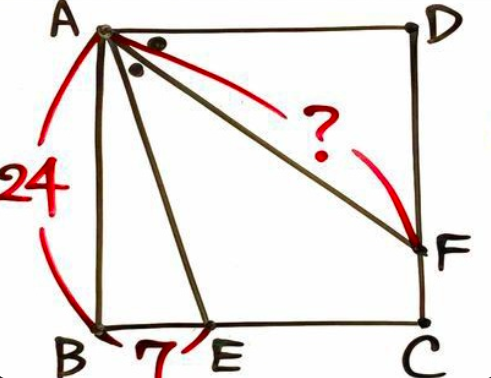
\includegraphics[scale=.4]{img/pythagore8.png}
\begin{tikzpicture}[scale=.2]
\tkzDefPoint(0,24){A}\tkzDefPoint(0,0){B}\tkzDefPoint(24,0){C}\tkzDefPoint(24,24){D}
\tkzDefPoint(7,0){E}
\tkzDrawPolygon[very thick](A,B,C,D)
\tkzDrawSegment(A,E)
\tkzDefLine[bisector](E,A,D) \tkzGetPoint{x}
\tkzInterLL(A,x)(D,C)\tkzGetPoint{F}
\tkzDrawSegment(A,F)
\tkzDrawPoints(E,F)
\tkzDefBarycentricPoint(A=1,C=1)\tkzGetPoint{O}
\tkzAutoLabelPoints[center=O](A,B,C,D,E,F)
\tkzMarkAngle[size=3,mark=|](E,A,F) \tkzMarkAngle[size=3,mark=|](F,A,D)
\tkzLabelSegment(B,A){$24$} \tkzLabelSegment(B,E){$7$} 
\end{tikzpicture}
\end{center}
\begin{sol}
Pythagore deux ou trois fois, projeter $E$ sur $[AF]$ (ou $F$ sur $AE$?) 
\end{sol}
\end{exo}


% - - - - - - - -
\begin{exo}
Dans un cercle $\mathcal C$, on a une corde $[AB]$ mesurant $4$cm. 
De plus, on sait que la distance entre le milieu de cette corde et le cercle est de $1$cm.
Quel est le rayon du cercle ?
\begin{center}
\begin{tikzpicture}
\tkzDefPoint(-2,0){A} \tkzDefPoint(2,0){B}
\tkzDefPoint(0,0){I} \tkzDefPoint(0,1){P}
\tkzDrawSegment(A,B)
\tkzDrawSegment[dashed](I,P)
\tkzDefPoint(0,-1.5){O}
\tkzDrawCircle[very thick](O,A)
\tkzLabelSegment[below](A,I) {$2$}
\tkzLabelSegment[below](I,B) {$2$}
\tkzLabelSegment[right](I,P) {$1$}
\tkzMarkRightAngle[size=.2](A,I,P)
\tkzDrawPoints(A,B,P)
\tkzLabelPoints[left](A) \tkzLabelPoints[right](B)
\end{tikzpicture}
\end{center}
\begin{hint}
Placer le centre $O$ du cercle. Que vaut la distance de $O$ à la corde, en fonction du rayon $R$ ?
Ensuite, on peut appliquer Pythagore.
\end{hint}
\begin{sol}
Le diamètre vaut $5$cm.
\end{sol}
\end{exo}



% - - - - - -

\begin{exo}
Dans un carré dont les côtés mesurent $1$cm, on inscrit un quart de cercle puis un petit cercle comme sur la figure.
Quel est le rayon du petit cercle ?
\begin{center}
\begin{tikzpicture}[scale=4]
\tkzDefPoint(0,0){O} \tkzDefPoint(1,0){A} \tkzDefPoint(1,1){B} \tkzDefPoint(0,1){C}
\tkzDefPoint(2*sqrt{2}-2,2*sqrt{2}-2){O'}
\tkzDefPoint(1/sqrt{2},1/sqrt{2}){P}
\tkzDrawPoint(O')
\tkzDrawArc[black,thick](O,A)(C)
\tkzDrawPolygon[very thick](O,A,B,C)
\tkzDrawCircle[black,thick](O',P)
\end{tikzpicture}
\end{center}
\begin{hint}
Tracer le centre du petit cercle et décomposer la diagonale du carré en plusieurs segments.
\end{hint}
\begin{sol}
On décompose la diagonale en trois segments : on obtient
\[ \sqrt 2 = 1+R+R\sqrt 2\]
Ceci aboutit à $R=3-2\sqrt{2}$.
\end{sol}
\end{exo}


% - - - - - - - - - - - - - - - - - - - - 


\begin{exo}
Quel est le rayon du cercle inscrit dans un triangle équilatéral de côté $1$cm?
Et si on rajoute trois petits cercles comme sur la figure de droite, quel est le rayon des petits cercles ?
\begin{center}
\begin{tikzpicture}[rotate=-30,scale=1.2]
\tkzDefPoint(0,0){O} \tkzDefPoint(0:2){A}\tkzDefPoint(120:2){B}\tkzDefPoint(240:2){C}
\tkzDefPoint(60:1){P}
\tkzDrawPolygon[very thick](A,B,C)
\tkzDrawCircle(O,P)
\end{tikzpicture}
\hspace{1cm}
\begin{tikzpicture}[rotate=-30,scale=1.2]
\tkzDefPoint(0,0){O}
\tkzDefPoint(0:2){A}\tkzDefPoint(120:2){B}\tkzDefPoint(240:2){C}
\tkzDefPoint(0:1){P}\tkzDefPoint(120:1){Q}\tkzDefPoint(240:1){R}
\tkzDefPoint(0:4/3){X} \tkzDefPoint(120:4/3){Y} \tkzDefPoint(240:4/3){Z}
\tkzDrawCircle(X,P)
\tkzDrawCircle(Y,Q)
\tkzDrawCircle(Z,R)
\tkzDrawPolygon[very thick](A,B,C)
\tkzDrawCircle(O,P)
\end{tikzpicture}
\end{center}
\begin{hint}
Il est peut-être plus simple de s'imaginer que le cercle est de rayon $1$ et de chercher la taille du triangle équilatéral.
Tracer les hauteurs de ce triangle équilatéral.
\end{hint}
\begin{sol}
On trouve $R=\frac{1}{2\sqrt 3}$. (Si le triangle est de côté $1$.)

Sinon, on peut remarquer que pour un triangle équilatéral, le centre du cercle inscrit est également le centre de gravité, ou le centre du cercle circonscrit. Il se trouve donc au tiers des médianes en partant de la base.
Or, les médianes sont les hauteurs, elles mesurent $\frac{\sqrt 3}{2}$.

Les petits cercles sont trois fois plus petits que le grand cercle, comme on le voit en traçant les tangentes communes aux cercles, ce qui partage le triangle en un hexagone de côté $1/3$ et trois petits triangles équilatéraux.

Comme on sait que $R=\frac{1}{2\sqrt 3}$, on trouve donc $r=\frac{1}{6\sqrt 3}$.
\end{sol}
\end{exo}






% - - - - - - -

\begin{exo}
Combien mesure le côté du triangle équilatéral, si les deux cercles ont un rayon de $1$cm ?
\begin{center}
\begin{tikzpicture}
\tkzDefPoint(-1-sqrt{3},0){A}\tkzDefPoint(1+sqrt{3},0){B}\tkzDefPoint(0,3+sqrt{3}){C}
\tkzDefPoint(-1,1){O} \tkzDefPoint(1,1){O'} \tkzDefPoint(0,1){P}
\tkzDrawCircle(O,P)
\tkzDrawCircle(O',P)
\tkzDrawPolygon[very thick](A,B,C)
\end{tikzpicture}
\end{center}
\begin{hint}
On peut tracer la hauteur qui passe entre les deux cercles et qui divise le triangle équilatéral en deux triangles rectangles. Combien mesure cette hauteur en fonction du côté du triangle ?
Ensuite, on peut se concentrer sur un seul de ces deux triangles, marquer les points de contact avec le cercle, et 
\end{hint}
\begin{sol}
On tracer la hauteur $CH$ comme indiqué, et on se concentre sur le triangle de gauche:
\begin{center}
\begin{tikzpicture}
\tkzDefPoint(-1-sqrt{3},0){A}\tkzDefPoint(1+sqrt{3},0){B}\tkzDefPoint(0,3+sqrt{3}){C}
\tkzDefPoint(-1,1){O} \tkzDefPoint(1,1){O'}
\tkzDefPoint(0,1){P}\tkzDefPoint(-1,0){Q} \tkzDefPoint(-1-sqrt{3}/2,1.5){R}
\tkzDefPoint(0,0){H}
\tkzDrawSegments[dashed](O,P O,Q O,R)
\tkzDrawCircle(O,P)
\tkzDrawPolygon[very thick](A,C,H)
\tkzDrawPoints(P,Q,R)
\tkzLabelSegments(Q,A){$x$} \tkzLabelSegments(A,R){$x$}
\tkzLabelSegments(P,H){$1$} \tkzLabelSegments(H,Q){$1$}
\tkzLabelSegments(R,C){$y$} \tkzLabelSegments(C,P){$y$}
\tkzAutoLabelPoints[center=O](A,C,H)
\end{tikzpicture}
\end{center}
La quantité que l'on cherche est $\ell = x+y$.



Appliquons Pythagore dans le triangle rectangle $ACH$, rectangle en $H$ : 
\[ (x+y)^2 = (y+1)^2+(x+1)^2,\]
c'est-à-dire, après simplification:
\[ xy = x+y+1\]
Comme il s'agit d'un triangle rectangle ayant des angles de $30^\circ$ et $60^\circ$, on sait (sinon on refait Pythagore) que le petit côté mesure la moitié de l'hypoténuse :
$x+y = 2(x+1)$, d'où on déduit que $y=x+2$.
En remplaçant $y$ par $x+2$ dans l'équation donnée par Pythagore, on obtient alors $x^2+2x = 2x+3$ donc $x=\sqrt{3}$.

Finalement, on obtient $\ell = x+y = 2x+2 = 2+2\sqrt 3$ pour la longueur du côté du triangle équilatéral.

\end{sol}
\end{exo}


% - - - - - - - -

\begin{exo}
Combien mesure le côté du triangle équilatéral, si les six cercles ont un rayon de $1$cm ?
(Généraliser ensuite avec plus de cercles : au lieu de six cercles, traiter le cas avec dix cercles, puis quinze etc.)
\begin{center}
\begin{tikzpicture}[scale=.8]
\def\ractrois{1.7320508076}
\draw (0,2*\ractrois) circle (1);
\draw (-1,\ractrois) circle (1);\draw (1,\ractrois) circle (1);
\draw (-2,0) circle (1); \draw (0,0) circle (1); \draw (2,0) circle (1);
\draw [very thick] (-2-\ractrois,-1) -- (2+\ractrois,-1) -- (0,2+2*\ractrois) -- cycle;
\end{tikzpicture}
\end{center}
\begin{hint}
On peut par exemple tracer es centres des cercles puis tracer le triangle qui relie les trois cercles extrémaux.
\end{hint}
\begin{sol}
\begin{center}
\begin{tikzpicture}[scale=.8]
\def\ractrois{1.7320508076}
\draw (0,2*\ractrois) circle (1);
\draw (-1,\ractrois) circle (1);\draw (1,\ractrois) circle (1);
\draw (-2,0) circle (1); \draw (0,0) circle (1); \draw (2,0) circle (1);
\draw  (-2-\ractrois,-1) -- (2+\ractrois,-1) -- (0,2+2*\ractrois) -- cycle;
\draw (-2,0) -- (2,0) -- (0,2*\ractrois) -- cycle;
\draw[very thick] (-2,-1) -- (-2,0) -- (-2-\ractrois,-1) -- cycle;
\draw[very thick] (2,-1) -- (2,0) -- (2+\ractrois,-1) -- cycle;
\end{tikzpicture}
\end{center}
Le triangle \og intérieur\fg, celui qui relie les centres des trois cercles extrémaux, fait $4$cm de côté.
Ensuite, il faut rajouter ce qui correspond aux deux petits triangles marqués sur la figure. 

Ces petits triangles sont des triangles rectangle avec des angles de $30^\circ$ et $60^\circ$ et un petit côté de $1$cm.
L'autre côté mesure donc $\sqrt 3$ (et l'hypoténuse mesure $2$cm).

Le grand triangle équilatéral a donc un côté qui mesure $4+2\sqrt 3$cm.

Généralisation : s'il y a $N$ cercles sur la rangée du bas, alors le côté est égal à $2N-2+2\sqrt 3$.
Il y a alors $\frac{N(N+1)}{2}$ cercles dans le triangle.
\end{sol}
\end{exo}






% - - - - - - - - - - - - - - - - - - - - 

\begin{exo}
Dans un rectangle de dimensions $3\mathrm{cm}\times 2\mathrm{cm}$, on inscrit deux demi-cercles de même rayon qui se touchent en un seul point, comme sur la figure.
Quel est le rayon de ces deux demi-cercles ? (Ce n'est pas $1$!)
\begin{center}
\begin{tikzpicture}[scale=2]
\draw[very thick] (0,0) rectangle (3,2);
\tkzDefPoint(13/12,0){O} \tkzDefPoint(23/12,2){O'} 
\tkzDefPoint(26/12,0){A} \tkzDefPoint(10/12,2){B} 
\tkzDrawSemiCircle(O,A)
\tkzDrawSemiCircle(O',B)
\tkzDrawPoints(O,O')
\tkzLabelPoints(O,O')
\end{tikzpicture}
\end{center}
\begin{sol}
On peut par exemple projeter le centre du rectangle sur une base, noter $x$ la distance de $O$ à ce projeté, et on obtient alors en considérant la largeur et la hauteur du rectangle :  $3=2R+2x$ et $2=2\sqrt{R^2-x^2}$, c'est-à-dire $1=R^2-x^2=\frac32(R-x)$, d'où finalement le système $R+x=\frac32$ et $R-x=\frac23$ et donc $2R=\frac{9+4}{6}$ et finalement $R=\frac{13}{12}$.

Autre méthode : on projette $O'$ sur la base, et on applique Pythagore dans $OO'H$. On a $OH=3-2R$, donc :
\[ (3-2R)^2+4=4R^2\]
Et donc $13-12R=0$, c'est plus rapide !
\end{sol}
\end{exo}





\begin{exo}[Cercles  tangents]
Les trois petits  cercles sont de rayon $1$.
Le grand cercle leur est simultanément tangent. Quel est son rayon ?
\begin{center}
\begin{tikzpicture}[scale=1]
\draw  (30:{2*sqrt(3)/3}) node {$R=1$}  circle (1);
\draw   (150:{2*sqrt(3)/3}) node {$R=1$} circle (1);
\draw  (270:{2*sqrt(3)/3}) node {$R=1$} circle (1);

\draw[very thick] (0,0) circle ({1+2*sqrt(3)/3});
% rajouter petit cercle ?
\end{tikzpicture}
\end{center}
\begin{hint}
Tracer le triangle (équilatéral) reliant les centres des trois petits cercles. Combien mesure  sa hauteur ?
\end{hint}
\end{exo}




\begin{exo}[Zig-zag dans un cercle]
Quel est le rayon du cercle ci-dessous ?
\begin{center}
\begin{tikzpicture}[scale=.5,rotate=20]
\draw  (0,0) circle ({2*sqrt(5)});
\draw[very thick] (-4,-2) node {$\bullet$}  node[below] {$A$} -- (-4,2) node {$\bullet$} node[left] {$B$} -- (2,2) node {$\bullet$} node[right] {$C$} -- (2,4) node {$\bullet$} node[above] {$D$};
\draw (-4,1.5) -- (-3.5,1.5) --(-3.5,2);
\draw (1.5,2) -- (1.5,2.5) -- (2,2.5);
\draw (-4,0) node[right] {$2$};
\draw (-1,2) node[below] {$3$};
\draw (2,3) node[right] {$1$};
\end{tikzpicture}
\end{center}
\begin{hint}
La droite $(BC)$ recoupe le cercle en  un point $E$. Que dire de $[AE]$ ?
L'objectif est de calculer la distance $CE$, après quoi le rayon du cercle est relativement rapide à obtenir.

Autre indication : il y a une racine carrée dans la réponse.
\end{hint}
\end{exo}

\begin{exo}[Zig-zag dans un cercle,bis]
Quel est le rayon du cercle ci-dessous ?
\begin{center}
\begin{tikzpicture}[scale=1,rotate=20]
\draw  (2.5,0) circle (2.5);
\draw[very thick] (0,0) node {$\bullet$}  node[left] {$A$} 
-- (1,0) node {$\bullet$} node[right] {$B$} node[midway, below] {$1$}
-- (1,2) node {$\bullet$} node[left] {$C$} node[midway, right] {$2$}
-- (4,2) node {$\bullet$} node[above] {$D$} node[midway, below] {$3$};

\draw (1,0) rectangle (.8,.2);
\draw (1,2) rectangle (1.2,1.8);

\end{tikzpicture}
\end{center}
\begin{hint}
La droite $(BC)$ recoupe le cercle en  un point $E$. Que dire de $[AE]$ ?
L'objectif est de calculer la distance $CE$, après quoi le rayon du cercle est relativement rapide à obtenir.
\end{hint}
\begin{sol}
Le diamètre est $5$.
\end{sol}
\end{exo}

\begin{exo}
Quatre carrés placés en damier sont inscrits dans un cercle qu'ils touchent en trois points, comme sur la figure.
Si les carrés mesurent chacun $1\mathrm{cm}^2$, quel est le rayon du cercle ?

\begin{center}
\begin{tikzpicture}[rotate=30]
\fill[color=gray] (0,0) rectangle (1,1);
\fill[color=gray] (1,1) rectangle (2,2);
\fill[color=gray] (1,2) rectangle (0,3);
\fill[color=gray]  (0,3) rectangle (-1,4);
\draw (.5,2.25) circle (sqrt{85}/4);
\draw (0,0) node {$\bullet$};
\draw (1,0) node {$\bullet$};
\draw (-1,4) node {$\bullet$};
\end{tikzpicture}
\end{center}
\begin{hint}
On peut trouver le centre en intersectant les médiatrices de deux cordes.
\end{hint}
\begin{sol}
Le rayon vaut $\sqrt{85}/4$.
\end{sol}
\end{exo}







% - - - - - - - - - - - - - - - - - - - - 

\begin{exo}[Triangle rectangle dans un quart de cercle]
Un triangle rectangle \og $3-4-5$\fg{} est inscrit dans un quart de cercle comme ci-dessous;
Quel est le rayon du quart de cercle ?
\begin{center}
\begin{tikzpicture}[scale=.8]
\draw (0,0) -- ({2*sqrt(5)},0) arc (0:90:{2*sqrt(5)}) -- cycle;
\draw[very thick] (0,{sqrt(5)}) node {$\bullet$} node[left] {$A$}
-- ({2*sqrt(5)},0) node[midway,fill=white] {$5$} node {$\bullet$} node[right] {$B$}
-- ({3*2*sqrt(5)/5},{sqrt(5)+3/sqrt(5)}) node[midway,fill=white] {$4$} node {$\bullet$} node[above] {$C$}
-- cycle node[midway,fill=white] {$3$}  ;
\end{tikzpicture}
\end{center}
% source : https://twitter.com/maliuhudmuaz/status/1315383186852118530 
\begin{hint}
On peut compléter la figure comme suit :
\begin{center}
\begin{tikzpicture}[scale=1]
\draw (0,0) -- ({2*sqrt(5)},0) arc (0:180:{2*sqrt(5)}) node[left] {$D$} node {$\bullet$} -- (0,0) -- (0,{2*sqrt(5)});
\draw[very thick] (0,{sqrt(5)}) node {$\bullet$} node[left] {$A$}
-- ({2*sqrt(5)},0) node[midway,fill=white] {$5$} node {$\bullet$} node[right] {$B$}
-- ({3*2*sqrt(5)/5},{sqrt(5)+3/sqrt(5)}) node[midway,fill=white] {$4$} node {$\bullet$} node[above] {$C$}
-- cycle node[midway,fill=white] {$3$}  ;
%\draw ({-2*sqrt(5)},0)-- (0,{sqrt(5)});
\end{tikzpicture}
\end{center}
Ensuite, on peut prolonger la droite $(AC)$.
\end{hint}
\begin{sol}
Complétons la figure comme suit :
\begin{center}
\begin{tikzpicture}[scale=1]
\draw (0,0) -- ({2*sqrt(5)},0) arc (0:180:{2*sqrt(5)}) node[left] {$D$} node {$\bullet$} -- (0,0) -- (0,{2*sqrt(5)});
\draw[very thick] (0,{sqrt(5)}) node {$\bullet$} node[left] {$A$}
-- ({2*sqrt(5)},0) node[midway,fill=white] {$5$} node {$\bullet$} node[right] {$B$}
-- ({3*2*sqrt(5)/5},{sqrt(5)+3/sqrt(5)}) node[midway,fill=white] {$4$} node {$\bullet$} node[above] {$C$}
-- cycle node[midway,fill=white] {$3$}  ;
\draw ({-2*sqrt(5)},0)-- (0,{sqrt(5)});
\end{tikzpicture}
\end{center}
Comme le triangle $ABC$ est rectangle en $C$, la droite $(AC)$ recoupe le droite $(OB)$ en $D$. Le triangle $DBC$ est rectangle en $C$ et on a $DC=8$ et $BC=4$, donc en appliquant le théorème de Pythagore, on obtient 
\[ DB=\sqrt{64+16}=\sqrt{80} = 4\sqrt5.\]
Le rayon est donc égal à $2\sqrt 5$.
\end{sol}
\end{exo}





%
%\begin{exo}
%\url{https://www.youtube.com/watch?v=og9Ak5ARqe4}
%
%Pas mal mais le rayon que 'on trouve est dégueu... Il faut faire trois fois pythagore.
%\end{exo}










% - - - - - - - - - - - - - - - - - - - - 

\begin{exo}[Le triangle $15^\circ-75^\circ-90^\circ$]
Le triangle $ABC$ a des angles qui mesurent $15^\circ$, $75^\circ$ et $90^\circ$, comme sur la figure ci-dessous. Son hypoténuse $AB$ mesure $1$ cm. 
Montrer que  $AC=\frac{\sqrt 3 +1}{2\sqrt 2}$ puis que $CB=\frac{\sqrt 3 - 1}{2\sqrt 2}$.

% en s'aidant des indications en pointillés sur la figure.

\begin{center}
\begin{tikzpicture}[scale=4]
\tkzDefPoint(-1,0){A}
\tkzDefPoint(0,0){B}
\tkzDefPoint(1,0){D}
\tkzDefPoint({sqrt(3)/2},1/2){E}
\tkzDefPoint({sqrt(3)/2},0){P}
\tkzDefPointBy[projection = onto A--E](B)
\tkzGetPoint{C}
\tkzDrawPolygon[very thick](A,B,C)
%\tkzDrawSegments[dashed](C,E B,E E,D E,P B,D)
%\tkzMarkRightAngles[size=.1](E,P,A A,C,B)
\tkzMarkRightAngles[size=.1](A,C,B)
%\tkzDrawSemiCircle[dashed](B,D)
\tkzLabelPoints[below left](A)
\tkzLabelPoints[below right](B)
\tkzDrawPoint(B)
\tkzLabelPoints[above](C)
\tkzLabelAngle[pos=.4](B,A,C){$15^\circ$}
\tkzLabelSegment[below](A,B){$1$}
\end{tikzpicture}
\end{center}
\begin{hint}
Attention, le calcul peut mener à des expressions qui \emph{semblent} différentes de celles demandées : il faut alors démontrer qu'elles coïncident avec les expressions demandées. Par exemple, on a $\sqrt{6+2\sqrt 5} = 1+\sqrt 5$. (Exercice : pourquoi ?)
\end{hint}
\begin{sol}
Considérer la symétrie axiale d'axe $(AC)$. 
On note $B'$ l'image de $B$ par cette symétrie.
Ensuite, projeter perpendiculairement le point $B$ sur la droite $(AB')$, et reconnaître un triangle rectangle ayant un angle de $30^\circ$ et une hypoténuse de $1cm$.
\end{sol}
\end{exo}



\begin{exo}[Consolidation : le triangle $22,5^\circ-67,5^\circ-90^\circ$]
Le triangle $ABC$ a des angles qui mesurent $22,5^\circ$, $67,5^\circ$ et $90^\circ$, comme sur la figure ci-dessous. Son hypoténuse mesure $1$ cm. 

En utilisant la même technique qu'au problème précédent, calculer $AC$.

\begin{center}
\begin{tikzpicture}[scale=5]
\clip (-1.5,.5) rectangle (.5,-.25);
\tkzDefPoint(-1,0){A}
\tkzDefPoint(0,0){B}
\tkzDefPoint(1,0){D}
\tkzDefPoint({sqrt(2)/2},{sqrt(2)/2}){E}
\tkzDefPoint({sqrt(2)/2},0){P}
\tkzDefPointBy[projection = onto A--E](B)
\tkzGetPoint{C}
\tkzDrawPolygon[very thick](A,B,C)
%\tkzDrawSegments[dashed](C,E B,E E,D E,P B,D)
%\tkzMarkRightAngles[size=.1](E,P,A  A,C,B)
%\tkzDrawSemiCircle[dashed](B,D)
\tkzLabelPoints[below left](A)
\tkzLabelPoints[below right](B)
\tkzDrawPoint(B)
\tkzLabelPoints[above](C)
\tkzLabelAngle[pos=.4](B,A,C){$22,5^\circ$}
\tkzLabelSegment[below](A,B){$1$}
\tkzMarkRightAngle[size=.1](A,C,B)
\end{tikzpicture}
\end{center}
\end{exo}



\begin{exo}
On inscrit trois cercles dans un demi-cercle de diamètre $8$cm, comme sur la figure ci-dessous. 
On note $A$ et $B$ le s points de contact du demi-cercle avec les deux petits cercles latéraux.
Combien mesure le segment $[AB]$ ?
\begin{center}
\begin{tikzpicture}
\tkzDefPoint(0,0){O} \tkzDefPoint(-sqrt{8},1){O'} \tkzDefPoint(sqrt{8},1){O''} \tkzDefPoint(0,2){I} 
\tkzDefPoint(4,0){P} \tkzDefPoint(-4,0){Q} 
\tkzDefPoint(-8*sqrt{2}/3,4/3){A} \tkzDefPoint(8*sqrt{2}/3,4/3){B} 
\tkzDrawSemiCircle[black,very thick](O,P)
\tkzDrawSegment[very thick](P,Q)
\tkzDrawCircle(I,O)
\tkzDrawCircle(O',A)\tkzDrawCircle(O'',B)
\tkzDrawPoints(A,B)
\tkzLabelPoint[above left](A){$A$} \tkzLabelPoint[above right](B){$B$}
\end{tikzpicture}
\end{center}
\begin{hint}
Notons $R$ le rayon des petits cercles, $O$ le centre du demi-cercle, $I$ le centre du grand cercle, $O'$ le centre du petit cercle latéral gauche, $C$ son projeté orthogonal sur la base du demi-cercle, $D$ son projeté orthogonal sur $(OI)$.
Appliquer Pythagore dans les triangles $OO'C$ et $O'DI$.
\end{hint}
\begin{sol}
En exprimant toutes les distances en fonction de $R$, les termes en $R^2$ s'annulent et on trouve une équation de degré un qui donne $R=1$.
Ensuite, on en déduit que $AB=16\sqrt 2 / 3$.

%Source :  vu par exemple sur la chaîne Math Booster, qui est pas trop mal : \url{https://www.youtube.com/watch?v=HbPQco5PVuU}
\end{sol}
\end{exo}



\begin{exo}[Olympiades polonaises]
Dans un demi-cercle de rayon $2$cm, on inscrit un premier demi-cercle deux fois plus petit, de rayon $1$cm, et un un cercle de rayon $R$, comme sur la figure.
Que vaut $R$ ?
\begin{center}
\begin{tikzpicture}[scale=1.5]
\tkzDefPoint(0,0){O}
\tkzDefPoint(2,0){P} \tkzDefPoint(-2,0){Q} 
\tkzDefPoint(-1,0){I} \tkzDefPoint(2/3,0){H}\tkzDefPoint(2/3,8/9){O'}
\tkzDrawSemiCircle[black,very thick](O,P)
\tkzDrawSegment[very thick](P,Q)
\tkzDrawSemiCircle[black](I,O)
\tkzDrawCircle(O',H)

\end{tikzpicture}
\end{center}
\begin{hint}

\end{hint}
\begin{sol}
On note $H$ le projeté du centre du petit cercle sur la base du grand demi-cercle.
On écrit Pythagore dans les deux triangles rectangles.
En notant $x=OH$, on trouve en éliminant $r^2$ l'équation $3r=2+x$.
On  injecte $x=3r-2$ dans la première équation, il reste $0=9r^2-8r$ d'où $r=8/9$.

%Source :  Olympiades polonaises, via Math booster \url{https://www.youtube.com/watch?v=KKzf3vh7-pY}
\end{sol}
\end{exo}








\begin{exo}
Dans un quart de cercle, on inscrit un demi-cercle comme sur la figure.
Si le rayon du demi-cercle est $1$cm, quel est le rayon du quart de cercle ?
\begin{center}
\begin{tikzpicture}[scale=2,rotate=135]
\tkzDefPoint(0,0){O}\tkzDefPoint(1,0){A} \tkzDefPoint(-1,0){B} 
\tkzDefPoint(1/sqrt{2},1/sqrt{2}){P} \tkzDefPoint(-1/sqrt{2},1/sqrt{2}){Q}
\tkzDrawSemiCircle[black](O,A)
\tkzDefPoint(0,sqrt{2}){O'}
\tkzInterLC(O',Q)(O',A)\tkzGetPoints{Y'}{Y}
\tkzInterLC(O',P)(O',A)\tkzGetPoints{X'}{X}
\tkzDrawArc[black, very thick](O',Y)(X)
\tkzDrawSegments(A,B)
\tkzDrawSegments[very thick](O',X O',Y)
% putain mais qu'est-ce qui m'a pris de faire la figure de cette façon...
\end{tikzpicture}
\end{center}
\begin{sol}
Le rayon du quart de cercle est $\sqrt 3$.
\end{sol}
\end{exo}




% - - - - - - - -
\begin{exo}[Théorème des lunules]
Soit $ABC$ un triangle rectangle en $C$. On trace le demi-cercle de diamètre $[AB]$ qui contient $C$ ainsi que les deux demi-cercles de diamètres $[BC]$ et $[CA]$ extérieurs au triangle. Ces trois demi-cercles délimitent deux lunules, coloriées en noir sur la figure.
Démontrer que la somme des aires de ces deux lunules est exactement égale à l'aire du triangle !
\begin{center}
\begin{tikzpicture}
\begin{scope}[rotate=atan(3/4)]
\draw[line width=1pt,fill=black,color=black] (0,3) arc (90:270:1.5cm) -- cycle;
\draw[line width=1pt,fill=black,color=black]   (0,0) arc (180:360:2cm) -- cycle;
\draw[line width=1pt,fill=white,color=white]  (0,3) arc (180-atan(3/4):360-atan(3/4):2.5cm) -- cycle;
\draw[line width=1pt] (0,0) -- (4,0) node[midway, fill=white] {$b$} -- (0,3) node[midway, fill=white] {$c$}-- cycle node[midway, fill=white] {$a$} ;
\draw (-.3,-.3) node {C};
\draw (4.3,.3) node {A};
\draw (.3,3.3) node {B};
\end{scope}
\end{tikzpicture}
\end{center}
\begin{hint}
Pour calculer l'aire des deux lunules, il faut calculer l'aire du demi-disque de diamètre $[AB]$ et la retrancher à une autre aire.
\end{hint}

\end{exo}


\section{Pythagore et triangles semblables}

\begin{exo}
% triangles semblables, aussi
Dans un triangle rectangle $ABC$ de type \og $3-4-5$\fg, on inscrit un demi-cercle comme sur la figure.
Calculer la distance $AP$.

\begin{center}
\begin{tikzpicture}[scale=1/7]
\tkzDefPoint(0,0){A} \tkzDefPoint(28,0){B} \tkzDefPoint(28,21){C} 
\tkzDefPoint(16-48/5,12-36/5){P}
\tkzDrawPolygon[very thick](A,B,C)
\tkzDefPoint(16,12){O} 
\tkzDrawSemiCircle[black](O,P)
\tkzMarkRightAngle[size=2](C,B,A)
\tkzDrawPoints(A,B,C,P)
\tkzLabelPoints[below left](A) \tkzLabelPoints[below right](B) \tkzLabelPoints[above right](C)
\tkzLabelPoints[above left](P)
\tkzLabelSegment[below](A,B){$4$}
\tkzLabelSegment[right](B,C){$3$}
\end{tikzpicture}
\end{center}
\end{exo}




\begin{exo}[Carrés dans un triangle 3-4-5]
% triangles semblables, aussi
Dans un triangle rectangle $ABC$ de type \og $3-4-5$\fg, on inscrit un carré de deux manières différentes, comme sur les deux figures.
Quelles sont les dimensions des deux carrés ?

\begin{center}
\begin{tikzpicture}[scale=1/7]
\tkzDefPoint(0,0){A} \tkzDefPoint(28,0){B} \tkzDefPoint(28,21){C} 
\tkzDrawPolygon[very thick](A,B,C)
\tkzDefPoint(16,12){O} \tkzDefPoint(16,0){P}  \tkzDefPoint(28,12){Q} 
\tkzDrawSegments(P,O O,Q)
\tkzMarkRightAngle[size=2](C,B,A)
\tkzLabelPoints[below left](A) \tkzLabelPoints[below right](B) \tkzLabelPoints[above right](C)
\end{tikzpicture}
\hspace{1cm}
\begin{tikzpicture}[scale=1/37]
\tkzDefPoint(0,0){A} \tkzDefPoint(148,0){B} \tkzDefPoint(148,111){C} 
\tkzDefPoint(100,0){P} \tkzDefPoint(148,36){Q}
\tkzDefSquare(P,Q)\tkzGetPoints{R}{S}
\tkzDrawPolygon(P,Q,R,S)
\tkzDrawPolygon[very thick](A,B,C)
\tkzMarkRightAngle[size=10](C,B,A)

\tkzLabelPoints[below left](A) \tkzLabelPoints[below right](B) \tkzLabelPoints[above right](C)
\end{tikzpicture}
\end{center}
\begin{sol}
Pour le deuxième carré, on a intérêt à noter $60x$ le côté du carré, de cette façon c'est divisible par $3$, $4$ et $5$. Ensuite on utilise les triangles semblables, mais du coup cet exo est faisable sans Pythagore. On trouve que $x=\frac{1}{37}$ par proportionnalité, le deuxième carré fait donc $60/37$ de côté.

Avec Pythagore ça doit être plus pénible...

Le première carré fait $12/7$ de côté. Là aussi, on a intérêt à noter $12y$ le côté, comme ça c'est divisible par trois et quatre. Et là aussi il vaut mieux faire ça avec des triangles semblables.
Il est plus gros que le premier car $444=12\times 37 \geq 7\times 60=420$. Sur le dessin ça se voir quand même assez nettement.
\end{sol}
\end{exo}






%
%\begin{exo}[]\url{https://twitter.com/archimedes_000/status/1524521121827151874} très bon
%\begin{center}
%\begin{tikzpicture}[scale=1]
%\end{tikzpicture}
%\end{center}
%\begin{hint}
%\end{hint}
%\end{exo}


\begin{exo}[Théorème de la hauteur relative à l'hypoténuse]
Soit $ABC$ un triangle rectangle en $C$ et $H$ le pied de la hauteur issue de $C$.
Montrer que 
\[ HA\times HB = HC^2.\]
\begin{center}
\begin{tikzpicture}[scale=.3]
\draw[very thick] (12,6) -- (15,0) -- (0,0) -- cycle;
\draw[dashed,thick] (12,0) -- (12,6);
\draw (0,0) node {$\bullet$} node[left] {A};
\draw (12,6) node {$\bullet$} node[above] {C};
\draw (15,0) node {$\bullet$} node[right] {B};
\draw (12,0) node {$\bullet$} node[below] {H};
\end{tikzpicture}
\end{center}
\begin{sol}
On fait Pythagore dans les trois triangles et ça se simplifie.

Évidemment on pourrait faire ça plus joliment avec des triangles semblables.
\end{sol}
\end{exo}





\begin{exo}[Inégalité arithmético-géométrique]
En utilisant l'exercice précédent, démontrer \emph{l'inégalité arithmético-géométrique}  : pour tous réels $x$ et $y$ positifs, on a 
\[ \sqrt{xy} \leq \frac{x+y}{2}.\]
(Le terme de gauche est la moyenne géométrique de $x$ et $y$, le terme de droite est leur moyenne arithmétique.) 
\end{exo}




\begin{exo}
Soit $ABC$ un triangle rectangle en $C$ et $H$ le pied de la hauteur issue de $C$.
Montrer que 
\[ \frac{1}{CH^2} = \frac{1}{BC^2}+\frac{1}{AC^2}.\]
\begin{center}
\begin{tikzpicture}[rotate=210]
\tkzDefPoint(0,3){A}
\tkzDefPoint(4,0){B}
\tkzDefPoint(0,0){C}
\tkzDefBarycentricPoint(A=1,B=1,C=1) \tkzGetPoint{G}
\tkzDefPointBy[projection=onto A--B](C) \tkzGetPoint{H}
\tkzDrawPolygon[very thick](A,B,C)
\tkzDrawSegment[dashed](C,H)
\tkzMarkRightAngle(C,H,B)
\tkzMarkRightAngle(A,C,B)
\tkzAutoLabelPoints[center=G](A,B,C,H)
%\tkzLabelSegment(B,C){$a$}
%\tkzLabelSegment(C,A){$b$}
%\tkzLabelSegment(C,H){$h$}
\end{tikzpicture}
\end{center}
\begin{hint}
Mettre au même dénominateur, éliminer les dénominateurs et calculer l'aire du triangle de deux façons.
\end{hint}
\end{exo}



\begin{exo}[Une corde]
Dans un cercle, une corde a pour longueur $2a$ et son milieu est à une distance $d$ du cercle.
Montrer que le diamètre du cercle est égal à $\frac{a^2+d^2}{d}$.
\begin{center}
\begin{tikzpicture}[scale=.5,rotate=20]
\tkzDefPoint(-4,3){A}
\tkzDefPoint(4,3){B}
\tkzDefPoint(0,5){C}
\tkzDefPoint(0,3){I}
\tkzDefPoint(0,0){O}

\tkzDrawSegment[very thick](A,B)
\tkzDrawSegment[dashed](I,C)
\tkzMarkRightAngle(C,I,B)
\tkzDrawCircle[thick](O,A)

\tkzDrawPoints(I,A,B,C,O)
\tkzLabelSegment[below](A,I){$a$}
\tkzLabelSegment[below](I,B){$a$}
\tkzLabelSegment[left](I,C){$d$}
\end{tikzpicture}
\end{center}
\end{exo}


\begin{exo}[Deux cordes parallèles]
Dans un cercle, deux cordes parallèles ont pour longueur $2a$ et $2b$. Elles sont distances d'une distance $d$.
Montrer que le rayon du cercle est égal à :
\[R=\frac{(d^2+(a-b)^2)(d^2+(a+b)^2)}{4d^2}.\]
\begin{center}
\begin{tikzpicture}[rotate=40]
\tkzDefPoint(-4,3){A}
\tkzDefPoint(4,3){B}
\tkzDefPoint(-3,4){A'}
\tkzDefPoint(3,4){B'}
\tkzDefPoint(0,3){M}
\tkzDefPoint(0,4){M'}
\tkzDefPoint(0,0){O}

\tkzDrawSegments[very thick](A,B A',B')
\tkzDrawSegment[dashed](M,M')
\tkzMarkRightAngles(A,M,M' M,M',A')
\tkzDrawArc[thick,delta=5](O,B)(A)

\tkzDrawPoints(M,M')
\tkzLabelSegment[below](A,M){$a$}
\tkzLabelSegment[below](M,B){$a$}
\tkzLabelSegment[above right](M,M'){$d$}
\tkzLabelSegment[above](A',M'){$b$}
\tkzLabelSegment[above](M',B'){$b$}
\end{tikzpicture}
\end{center}
\end{exo}

\begin{exo}
Une ligne brisée $ABCD$ à angles droits est inscrite dans un demi-cercle.
Quel est le rayon du demi-cercle ?
\begin{center}
\begin{tikzpicture}[scale=1.2]
\tkzDefPoint(-1,2){A}
\tkzDefPoint(-1,0){B}
\tkzDefPoint(2,0){C}
\tkzDefPoint(2,1){D}
\tkzDrawSegments[very thick](A,B B,C C,D)


\tkzDefPoint(0,0){O}
\tkzInterLC(B,C)(O,A)
\tkzGetPoints{a}{b}
\tkzDrawSegment[thick](a,b)
\tkzDrawSemiCircle[thick](O,b)

\tkzMarkRightAngles(A,B,C B,C,D)
\tkzDrawPoints(A,B,C,D)
\tkzLabelSegment[left](A,B){$2$}
\tkzLabelSegment[below](B,C){$3$}
\tkzLabelSegment[left](C,D){$1$}
\tkzLabelPoints[above left](A)
\tkzLabelPoints[below left](B)
\tkzLabelPoints[below right](C)
\tkzLabelPoints[above right](D)
\end{tikzpicture}
%
%\definecolor{ududff}{rgb}{0.30196078431372547,0.30196078431372547,1.}
%\definecolor{uuuuuu}{rgb}{0.26666666666666666,0.26666666666666666,0.26666666666666666}
%\definecolor{xdxdff}{rgb}{0.49019607843137253,0.49019607843137253,1.}
%\begin{tikzpicture}[line cap=round,line join=round,>=triangle 45,x=1.0cm,y=1.0cm]
%\clip(-4.3,-7.24) rectangle (12.28,6.3);
%\draw [line width=2.pt] (0.,4.)-- (0.,0.);
%\draw [line width=2.pt] (6.,0.)-- (6.,2.);
%\draw [shift={(2.,0.)},line width=2.pt]  plot[domain=0.:3.141592653589793,variable=\t]({1.*4.47213595499958*cos(\t r)+0.*4.47213595499958*sin(\t r)},{0.*4.47213595499958*cos(\t r)+1.*4.47213595499958*sin(\t r)});
%\draw [line width=2.pt] (-2.4721359549995796,0.)-- (6.47213595499958,0.);
%\draw [line width=2.pt] (0.,0.)-- (6.,0.);
%\begin{scriptsize}
%\draw [fill=xdxdff] (0.,4.) circle (2.5pt);
%\draw[color=xdxdff] (0.14,4.37) node {$A$};
%\draw [fill=uuuuuu] (0.,0.) circle (2.0pt);
%\draw[color=uuuuuu] (0.,-0.35) node {$B$};
%\draw [fill=xdxdff] (6.,0.) circle (2.5pt);
%\draw[color=xdxdff] (6.12,-0.33) node {$C$};
%\draw [fill=ududff] (6.,2.) circle (2.5pt);
%\draw[color=ududff] (6.14,2.37) node {$D$};
%\draw[color=black] (-0.26,2.19) node {4};
%\draw[color=black] (5.52,1.19) node {2};
%\draw[color=black] (3.06,-0.13) node {6};
%\end{scriptsize}
%\end{tikzpicture}


%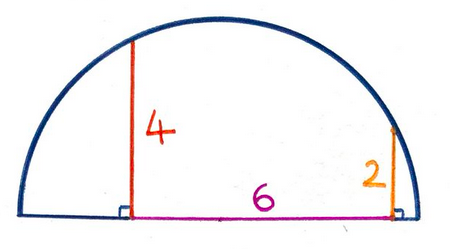
\includegraphics[scale=.4]{pythagore3.png}
\end{center}
\end{exo}



\begin{exo}
Soit $ABC$ un triangle avec $\widehat{A}=60^\circ$ et $\widehat{B}=45^\circ$. 
Calculer $\frac{CA}{CB}$.
\begin{center}
\begin{tikzpicture}[scale=.8]
\tkzDefPoint(0,0){A}
\tkzDefPoint(5,0){B}
\tkzDefPointBy[rotation=center A angle 60](B) \tkzGetPoint{B'}
\tkzDefPointBy[rotation=center B angle -45](A) \tkzGetPoint{A'}
\tkzInterLL(A,B')(B,A')\tkzGetPoint{C}
\tkzDefBarycentricPoint(A=1,B=1,C=1) \tkzGetPoint{G}

\tkzDrawPolygon[very thick](A,B,C)
\tkzLabelAngle(B,A,C){$60^\circ$}
\tkzLabelAngle(C,B,A){$45^\circ$}
\tkzAutoLabelPoints[center=G](A,B,C)
%\tkzDrawPoints(A,B,C,A',B')
\end{tikzpicture}
%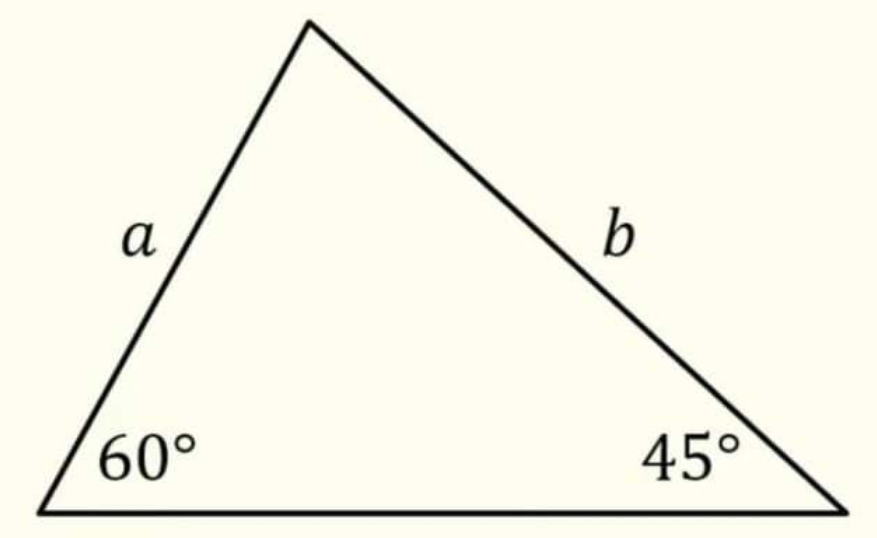
\includegraphics[scale=.4]{pythagore5.png}
\end{center}
\begin{sol}
Projeter $C$ sur $[AB]$ et appliquer Pythagore deux fois.
\end{sol}
\end{exo}




\begin{exo}
Dans un triangle rectangle en $A$, en notant $H$ le pied de la hauteur issue de $A$, on a $AB=15$ et $HC=16$.
Calculer $BH$, $AH$ et $AC$.
\begin{center}
\begin{tikzpicture}[scale=1/4]
\tkzDefPoint(0,0){H} \tkzDefPoint(0,12){A} \tkzDefPoint(-9,0){B} \tkzDefPoint(16,0){C}
\tkzDrawPolygon[very thick](A,B,C)
\tkzDrawSegment[dashed](A,H)
\tkzLabelPoints[above](A) \tkzLabelPoints[left](B) \tkzLabelPoints[right](C) \tkzLabelPoints[below](H)
\tkzDrawPoint(H)
\tkzMarkRightAngle[size=1](A,H,B) \tkzMarkRightAngle[size=1](B,A,C)
\tkzLabelSegment[above left](A,B){$15$} \tkzLabelSegment(H,C){$16$} 
\end{tikzpicture}
\end{center}
\begin{sol}
En calculant l'aire du triangle de deux façons, on a $AH\times BC = AB\times AC$.

Ensuite, on peut procéder de plusieurs façons, juste avec Pythagore dans les trois triangles rectangles, ou en remarquant des triangles semblables.
Par exemple, comme $ABH$ et $CAH$ sont semblables, on a, par proportionnalité, le produit en croix $AH^2=HB\times HC = 16 HB$.

Ensuite, en appliquant le théorème de Pythagore dans le triangle $ABH$ rectangle en $H$, on obtient:
\[ 15^2 = AH^2+BH^2 = 16BH+BH^2 = (BH+8)^2-64\]
On en tire $BH+8=\sqrt{15^2+8^2}=\sqrt{289}=17$, d'où $BH=17-8=9$.

Ensuite, on continue et on trouve normalement $AH=12$ et $AC=20$.
\end{sol}
\end{exo}






\begin{exo}[Théorème des cordes sécantes dans un cas particulier]
Dans un cercle, on trace une corde $[AB]$, de milieu $M$. Sa médiatrice intersecte le cercle en $C$ et $D$.
Montrer que
\[ MA\times MB = MC\times MD.\]
\begin{center}
\begin{tikzpicture}[rotate=50,scale=.8]
\tkzDefPoint(-2,0){A} \tkzDefPoint(2,0){B}
\tkzDefPoint(0,1){C} \tkzDefPoint(0,-4){D}
 \tkzDefPoint(0,0){M} 
\tkzDrawSegment(A,B)
\tkzDrawSegment(C,D)
\tkzDefPoint(0,-1.5){O}
\tkzDrawCircle[very thick](O,A)
\tkzMarkRightAngle[size=.2](A,M,C)
\tkzDrawPoints(A,B,C,D,M)
\tkzLabelPoints[left](A) \tkzLabelPoints[right](B)\tkzLabelPoints[left](C) \tkzLabelPoints[right](D)\tkzLabelPoints[above](M)
\tkzMarkSegment[mark=||](A,M)
\tkzMarkSegment[mark=||](M,B)
\end{tikzpicture}
\end{center}
(Note : en réalité, ce théorème reste vrai pour deux cordes \emph{quelconques} s'intersectant en $M$, mais la démonstration est plus difficile et utilise le théorème de l'angle inscrit. La quantité $MA\times MB$ est alors appelée la \emph{puissance} du point $M$ par rapport au cercle.)
\end{exo}









\begin{exo}
Sur un demi-cercle de diamètre $[AC]$, on place un point $M$ de sorte à avoir les longueurs $HB=3$ et $HM=6$. Quel est le rayon du demi-cercle ?
\begin{center}
\begin{tikzpicture}[scale=.3]
\draw[thick] (15,0) -- (0,0) ;
\draw[thick] (12,0) -- (12,6);
\draw[thick] (11,0) -- (11,1) -- (12,1);
\draw[thick] (15,0) arc (0:180:7.5cm);
\draw (13.5,0) node[above] {$3$} ;
\draw (12,3) node[left] {$6$} ;
\draw (0,0) node {$\bullet$} node[left] {A};
\draw (12,0) node {$\bullet$} node[below] {H};
\draw (15,0) node {$\bullet$} node[right] {B};
\draw (12,6) node {$\bullet$} node[below] {M};
\end{tikzpicture}
\end{center}
\begin{sol}
Source : \url{https://twitter.com/Math_World_/status/1519662926860365824}

On peut utiliser le théorème de la hauteur relative à l'hypoténuse (citer référence du problème).

On peut aussi refaire trois fois Pythagore, (ou bien utiliser les triangles semblables, ou utiliser la puissance du point $K$ par rapport au cercle.)
\end{sol}
\end{exo}










\section{Circle Packing}

\begin{exo}[circle packing, 1]
Les trois cercles ci-dessous sont tangents et inscrits dans un rectangle. Leurs diamètres valent $3$, $4$ et $6$.
Calculer la longueur $AB$.
\begin{center}
\begin{tikzpicture}[scale=.5]
\draw[very thick] (-1.5,0) rectangle ({3+3*sqrt(6)},6);
\draw  (0,1.5) circle (1.5);
\draw ({3*sqrt(6)},3) circle (3);
\draw ({sqrt(6)},4) circle (2);
\draw (0,0) node {$\bullet$} node[below] {$A$};
\draw ({3*sqrt(6)},0) node {$\bullet$} node[below] {$B$};
\end{tikzpicture}
\end{center}
\begin{hint}
\end{hint}
\begin{sol}
On obtient $AB=\sqrt 6 + 2\sqrt 6 = 3\sqrt 6$. (on fait deux fois Pythagore)
\url{https://twitter.com/0y6tr4/status/1521866673493618690} 
\end{sol}
\end{exo}



\begin{exo}[Cercles dans un carré ]
La figure suivante représente des cercles qui ont  un rayon égal à $1$ et placés dans un carré.
Quelles sont les dimensions des carrés ?
\begin{center}

\begin{tikzpicture}[scale=1]
\draw[thick] ({1/sqrt(2)},{1/sqrt(2)}) circle (1.cm);
\draw[thick] ({-1/sqrt(2)},{-1/sqrt(2)}) circle (1.cm);
\draw [very thick] ({-1-sqrt(2)/2},{-1-sqrt(2)/2}) rectangle ({1+sqrt(2)/2},{1+sqrt(2)/2});
\end{tikzpicture}
\hspace{1cm}
\begin{tikzpicture}[line cap=round,line join=round,>=triangle 45,scale=1]
\draw[thick] (1.,1.) circle (1.cm);
\draw [thick] (1.517638090205042,2.931851652578137) circle (1.cm);
\draw [thick] (2.931851652578137,1.5176380902050417) circle (1.cm);
\draw [very thick] (0.,0.)-- (3.932,0.) -- (3.932,3.932)-- (0,3.932) -- cycle;
\end{tikzpicture}
\end{center}
\begin{hint}

\end{hint}
\begin{sol}
\url{https://erich-friedman.github.io/packing/cirinsqu/}
VERIFIER Le carré est de côté $2+\frac{1}{\sqrt 2} + \frac{\sqrt 6}{2}$.

Pour le premier le côté vaut $2+\sqrt2$.
\end{sol}
\end{exo}


\begin{exo}[Cercles dans un carré, bis ]
La figure suivante représente des cercles qui ont  un rayon égal à $1$ et placés dans un carré.
Quelles sont les dimensions du carré ?
\begin{center}

\begin{tikzpicture}[scale=1]
\draw[thick] (0,0) circle (1.cm);
\draw[thick] (0,{8/sqrt(13)}) circle (1.cm);

\draw[thick] ({-6/sqrt(13)},{4/sqrt(13)}) circle (1.cm);
\draw[thick] ({-6/sqrt(13)},{-4/sqrt(13)}) circle (1.cm);
\draw[thick] ({6/sqrt(13)},{4/sqrt(13)}) circle (1.cm);
\draw[thick] ({6/sqrt(13)},{-4/sqrt(13)}) circle (1.cm);
\draw [very thick] ({-6/sqrt(13)-1},{-4/sqrt(13)-1}) rectangle ({6/sqrt(13)+1},{8/sqrt(13)+1}) ;
\end{tikzpicture}

\end{center}
Note : il s'agit du plus petit carré qui peut contenir six disques de rayon un. Ce résultat a été prouvé par Graham en 1963.
\begin{hint}

\end{hint}
\begin{sol}
Le carré a un côté de $2+\frac{12}{\sqrt 13}$. Voir la vidéo \url{https://www.youtube.com/watch?v=ONs1u3xRzrM&t=12s} et bien sûr le site \url{https://erich-friedman.github.io/packing/cirinsqu/}.
\end{sol}
\end{exo}



\section{Square packing}







\begin{exo}[Cinq carrés dans un carré]
On cherche à placer cinq petits carrés identiques de $1\mathrm{cm}^2$ dans un grand carré, de la façon la plus \og efficace\fg{} possible.

Les deux figures ci-dessous présentent deux configurations possibles. On arrive à voir à l'\oe il nu que la seconde configuration est la plus efficace des deux.
Démontrer ce résultat en calculant dans les deux cas les dimensions du grand carré.

\begin{center}

\begin{tikzpicture}[scale=1]
\begin{scope}[rotate=45,shift={(-1.5,-.5)}]
\draw[fill=gray] (0,0) rectangle (3,1);
\draw[fill=gray] (1,-1) rectangle (2,0);
\draw[fill=gray] (1,0) rectangle (2,1);
\draw[fill=gray] (1,1) rectangle (2,2);
\end{scope}
\draw[very thick] (-1.42,-1.42) rectangle (1.42,1.42);
\end{tikzpicture}
\hspace{1cm}
\begin{tikzpicture}[scale=1]
\draw[fill=gray] ({sqrt(2)/4},{sqrt(2)/4}) rectangle ({1+sqrt(2)/4},{1+sqrt(2)/4});
\draw[fill=gray] ({-sqrt(2)/4},{sqrt(2)/4}) rectangle ({-1-sqrt(2)/4},{1+sqrt(2)/4});
\draw[fill=gray] ({sqrt(2)/4},{-sqrt(2)/4}) rectangle ({1+sqrt(2)/4},{-1-sqrt(2)/4});
\draw[fill=gray] ({-sqrt(2)/4},{-sqrt(2)/4}) rectangle ({-1-sqrt(2)/4},{-1-sqrt(2)/4});
\draw[fill=gray] ({-sqrt(2)/2},0)  -- (0,{sqrt(2)/2}) -- ({sqrt(2)/2},0) -- (0,{-sqrt(2)/2}) -- cycle;
\draw[very thick] ({-1-sqrt(2)/4},{-1-sqrt(2)/4}) rectangle ({1+sqrt(2)/4},{1+sqrt(2)/4});
\end{tikzpicture}
\end{center}
Note : Frits Göbel a prouvé en 1979 que la configuration de droite est la plus efficace parmi toutes les manières de placer cinq carrés dans un carré.

\begin{hint}
\end{hint}
\begin{sol}
\url{https://erich-friedman.github.io/packing/squinsqu/}
\end{sol}
\end{exo}


\begin{exo}[Dix carrés dans un carré]
Pour dix petits carrés, le plus petit carré est le suivant, mais ça n'a été démontré qu'en 2003 par Walter Stromquist. Quelle est la taille du carré ? (Les carrés obliques sont toujours  inclinés de $45^\circ$.)
\begin{center}
\begin{tikzpicture}[scale=1]

%\draw[fill=gray] ({sqrt(2)/4},{sqrt(2)/4}) rectangle ({1+sqrt(2)/4},{1+sqrt(2)/4});
\draw[fill=gray] ({-sqrt(2)/4},{sqrt(2)/4}) rectangle ({-1-sqrt(2)/4},{1+sqrt(2)/4});
\draw[fill=gray] ({sqrt(2)/4},{-sqrt(2)/4}) rectangle ({1+sqrt(2)/4},{-1-sqrt(2)/4});
\draw[fill=gray] ({-sqrt(2)/4},{-sqrt(2)/4}) rectangle ({-1-sqrt(2)/4},{-1-sqrt(2)/4});

\draw[fill=gray] ({-sqrt(2)/4},{1+sqrt(2)/4}) rectangle ({-1-sqrt(2)/4},{2+sqrt(2)/4});
\draw[fill=gray] ({1-sqrt(2)/4},{1+sqrt(2)/4}) rectangle ({-sqrt(2)/4},{2+sqrt(2)/4});

\draw[fill=gray] ({1+sqrt(2)/4},{-sqrt(2)/4}) rectangle ({2+sqrt(2)/4},{-1-sqrt(2)/4});
\draw[fill=gray] ({1+sqrt(2)/4},{1-sqrt(2)/4}) rectangle ({2+sqrt(2)/4},{-sqrt(2)/4});

\draw[fill=gray] ({1+sqrt(2)/4},{1+sqrt(2)/4}) rectangle ({2+sqrt(2)/4},{2+sqrt(2)/4});

\draw[fill=gray] ({-sqrt(2)/2},0)  -- (0,{sqrt(2)/2}) -- ({sqrt(2)/2},0) -- (0,{-sqrt(2)/2}) -- cycle;
\draw[fill=gray]  (0,{sqrt(2)/2}) -- ({sqrt(2)/2},0) -- ({sqrt(2)},{sqrt(2)/2}) -- ({sqrt(2)/2},{sqrt(2)})  --cycle;

\draw[very thick] ({-1-sqrt(2)/4},{-1-sqrt(2)/4}) rectangle ({2+sqrt(2)/4},{2+sqrt(2)/4});
\end{tikzpicture}
\end{center}
Ces problèmes pourraient sembler évidents mais ne le sont pas. Par exemple, pour $11$ carrés, on a longtemps cru que la configuration optimale était celle ci-dessous à gauche, avec des carrés inclinés à $45^\circ$.
Mais en 1979, Walter Trump trouva une autre configuration légèrement meilleure, avec un angle d'environ $40,18^\circ$. On ignore encore si cette dernière configuration est optimale !
\begin{center}
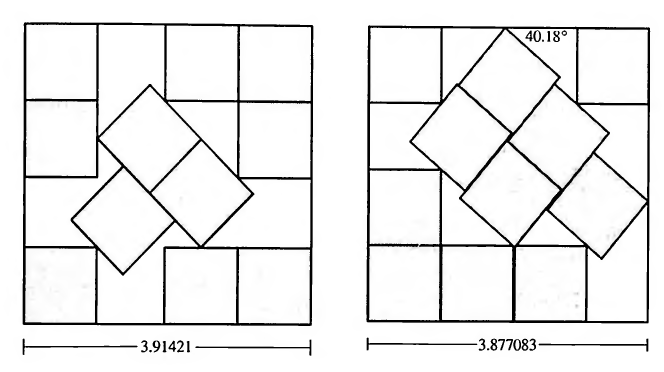
\includegraphics[scale=.4]{sqinsq/11squares_comp.png}\\
Illustration tirée du livre \emph{Which Way Did The Bycicle Go ?}, p. 105.
\end{center}

Pour $17$ carrés, la meilleure configuration connue à ce jour est la suivante. On connaît finalement assez peu de choses sur ces questions !
\begin{center}
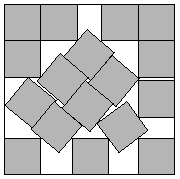
\includegraphics[scale=.5]{sqinsq/s17.png}
\end{center}
\begin{hint}
\end{hint}
\begin{sol}
\url{https://erich-friedman.github.io/packing/squinsqu/}
\end{sol}
\end{exo}









%\begin{exo}[]\url{https://twitter.com/archimedes_000/status/1524521121827151874} très bon
%\begin{center}
%\begin{tikzpicture}[scale=1]
%\end{tikzpicture}
%\end{center}
%\begin{hint}
%\end{hint}
%\end{exo}




\begin{exo}[Vers le théorème de Descartes]
Les trois grands  cercles sont de rayon $1$ et $2$.
Le petit cercle leur est simultanément tangent. Quel est son rayon ?
\begin{center}
\begin{tikzpicture}[rotate=90,scale=1.1]
\draw (-1,0) node {$R=1$}  circle (1);
\draw (1,0) node {$R=1$}  circle (1);
\draw (0,{2*sqrt(2)}) node {$R=2$}  circle (2);
\begin{scriptsize}
\draw[very thick] (0,{2*sqrt(2)-2-(32*sqrt(2)-40)/(28)}) node {$?$} circle ({(32*sqrt(2)-40)/(28)});
\end{scriptsize}
\end{tikzpicture}
\end{center}
\begin{hint}
Tracer les centres des cercles et les relier.
\end{hint}
\end{exo}

%- - - - - - - - - -

\begin{exo}[Cercles de Ford]
Sur une droite graduée, on \og pose\fg{} des cercles de diamètre $\frac{1}{n^2}$ sur les abscisses $\frac{1}{n}$, comme sur la figure ci-dessous. Montrer que tous ces cercles sont tangents, et qu'ils sont tous tangents au cercle de diamètre $1$ posé en l'origine !!
\begin{center}
\begin{tikzpicture}[scale=9]
\clip (-.15,-.1) rectangle (.7,.4);
\draw[very thick] (-0.2,0) -- (.6,0);
\draw (0,0) node[below] {$0$};

\foreach \i in {2, 3, 4, 5, 6, 7}
{
\draw  ({1/\i},{1/(2*\i*\i)}) circle ({1/(2*\i*\i)});
\draw ({1/\i},0) node {$\bullet$} node[below] {$\frac{1}{\i}$};
}

\draw[dashed] (0,1/2) circle (1/2);
\draw (0,0) node {$\bullet$};
\end{tikzpicture}
\end{center}
\begin{hint}
Commencer par montrer que les deux premiers cercles, de diamètres $1/4$ et $1/9$, sont tangents. Dessiner leurs centres.
\end{hint}
\end{exo}


\section{Théorèmes classiques démontrés avec Pythagore}


\begin{exo}[Premier théorème de la médiane (théorème d'Apollonius)]
%\url{https://www.youtube.com/watch?v=pqHpU84ggpY}
Soit $ABC$ un triangle et $I$ le milieu de $[BC]$.
Établir les deux identités (équivalentes) suivantes :
\[ 2AB^2+2AC^2 = BC^2+4AI^2\]
\[ AB^2+AC^2 = 2BI^2+2AI^2\]
\begin{center}
\begin{tikzpicture}
\tkzDefPoint(.5,3){A}\tkzDefPoint(0,0){B}\tkzDefPoint(4,0){C}
\tkzDefBarycentricPoint(B=1,C=1)\tkzGetPoint{I}
%\tkzDefPointBy[projection = onto B--C](A) \tkzGetPoint{H}
\tkzDrawPolygon[very thick](A,B,C)
\tkzDrawSegment[dashed](A,I)
\tkzMarkSegment[mark=||](B,I)\tkzMarkSegment[mark=||](I,C)
\tkzDrawPoint(I)
\tkzLabelPoint[above](A){$A$}\tkzLabelPoint[below left](B){$B$}\tkzLabelPoint[below right](C){$C$}\tkzLabelPoint[below](I){$I$}
\end{tikzpicture}
\end{center}
\begin{hint}
On peut par exemple démontrer la seconde identité pour commencer.
(Conseil : noter les longueurs $a$, $b$, $c$, $h$ et $m$, par exemple. Et on peut noter $BI : a/2 = a'$. Ainsi on veut démontrer 
 que $b^2+c^2 = 2m^2+2a'^2$.)
Considérer la hauteur $[AH]$ issue de $A$ et utiliser Pythagore dans les trois triangles $AHB$, $AHI$ et $AHC$. Puis, exprimer toutes les quantités inconnues autres que les côtés du triangle en fonction de $AI$ et $BI$. 
\end{hint}
\end{exo}


\begin{exo}[Identité du parallélogramme]
Soit $ABCD$ un parallélogramme.
Montrer que
\[ AC^2+BD^2 = 2AB^2+2BC^2\]
\begin{center}
\begin{tikzpicture}
\end{tikzpicture}
\end{center}
\begin{hint}
Utiliser le premier théorème de la médiane. Sinon, on peut refaire le travail en projetant un sommet du parallélogramme sur une diagonale.
\end{hint}
\begin{sol}
Il y a aussi une rédaction courte ici \url{https://math.stackexchange.com/questions/3185755/parallelogram-law-geometric-proof} avec Pythagore.
\end{sol}
\end{exo}


\begin{exo}[Troisième théorème de la médiane]
Soit $ABC$ un triangle,  $I$ le milieu de $[BC]$ et $H$ le pied de la hauteur issue de $A$.
En supposant que $I$ est dans le segment $[BI]$ comme sur la figure ci-dessous, montrer que 
\[ AC^2-AB^2 = 2BC\times IH.\]
Et si la hauteur n'appartient pas au segment $[BI]$? 
% C'est  \[ |AC^2-AB^2| = 2BC\times IH.\]
\begin{center}
\begin{tikzpicture}
\tkzDefPoint(.5,3){A}\tkzDefPoint(0,0){B}\tkzDefPoint(4,0){C}
\tkzDefBarycentricPoint(B=1,C=1)\tkzGetPoint{I}
\tkzDefPointBy[projection = onto B--C](A) \tkzGetPoint{H}
\tkzDrawPolygon[very thick](A,B,C)
\tkzDrawSegment[dashed](A,I)
\tkzDrawSegment[dashed](A,H)
%\tkzMarkSegment[mark=||](B,I)\tkzMarkSegment[mark=||](I,C)
\tkzDrawPoint(I)\tkzDrawPoint(H)
\tkzMarkRightAngle[size=.2](I,H,A)
\tkzLabelPoint[above](A){$A$}\tkzLabelPoint[below left](B){$B$}\tkzLabelPoint[below right](C){$C$}
\tkzLabelPoint[below](I){$I$}\tkzLabelPoint[below](H){$H$}
\end{tikzpicture}
\end{center}
\begin{hint}

\end{hint}
\end{exo}


%Plus difficile, avec trinôme et factoriastion : 
%\url{https://www.youtube.com/watch?v=KKzf3vh7-pY}



\begin{exo}[Formule de Héron]
\begin{center}
\begin{tikzpicture}
\end{tikzpicture}
\end{center}
\begin{hint}
\end{hint}
\begin{sol}
\end{sol}
\end{exo}



\begin{exo}[Loi des cosinus (Al-Kashi)]
\begin{center}
\begin{tikzpicture}
\end{tikzpicture}
\end{center}
\begin{hint}
\end{hint}
\begin{sol}
\end{sol}
\end{exo}





\begin{exo}[Loi des sinus]
\begin{center}
\begin{tikzpicture}
\end{tikzpicture}
\end{center}
\begin{hint}
\end{hint}
\begin{sol}
\end{sol}
\end{exo}





\begin{exo}
\begin{center}
\begin{tikzpicture}
\end{tikzpicture}
\end{center}
\begin{hint}
\end{hint}
\begin{sol}
\end{sol}
\end{exo}


\section{Autre}



\begin{exo}[Comparaisons de racines carrées]

On considère les trois nombres suivants : $A=3+\sqrt 2$, $B=\sqrt 5 +\sqrt 6$ et $C=1+\sqrt 10$ ?
Classer ces trois nombres du plus petit au plus grand, sans utiliser évidemment de calculatrice.
\begin{hint}
Élever les trois quantités au carré.
\end{hint}
\begin{sol}
On a 
\[
A^2 = 11+6\sqrt 2 = 11+\sqrt{72},\quad
B^2 = 11+2\sqrt{30}=11+\sqrt{120} \quad\text{et}
C^2 = 11+2\sqrt{10}=11+\sqrt{40}.\]
On en déduit que 
\[ C< A < B.\]
\end{sol}
\end{exo}




\Closesolutionfile{indications}
\Closesolutionfile{solutions}

\indications
\correction

\end{document}

